\documentclass{inets-thesis}

% For editing the LaTeX environment, refer to owndefs.tex. Don't edit the inets-thesis.cls file!

% Title of the thesis
\ThesisTitle{Coexistence Study of Different Medium Access Mechanisms Using a Software Defined Radio Testbed}

% Thesis type ("M" = master thesis, "B" = bachelor thesis)
\ThesisType{B}

% Author's name (firstname(s) lastname)
\ThesisAuthor{Alexander Pastor}

% Date (year month day)
\ThesisDate{2017}{10}{24}

% Examiners: Check who is your first examiner from our professors.
% There is always one first examiner (listed in your registration sheet), and one more examiner
% who in our case is usually the respective other professor, supervisors are non-faculty members
% who supported you in addition to the first examiner in the development of the thesis
% Advisers: Reference with name and title, note that old German titles (Dipl.-Ing.) and doctor titles (Dr. or % Dr.-Ing.) are prefix while ``M.Sc.'' is a postfix to the name of the person
\FirstExaminerName{Prof.~Dr.~Petri M\"ah\"onen}
\SecondExaminerName{Prof.~Dr.-Ing.~Marina Petrova}
\SupervisorNames{Peng~Wang,~M.Sc.\\Andra~Voicu,~M.Sc.}

\begin{document}

%\chapter{First Chapter Heading}

Use\footnote{This is a footnote to the word ``use''.}
\emph{The Not So Short Introduction to \LaTeXe}~\cite{Oetiker00}
to familiarize yourself with \LaTeX. When citing research papers, use a protected space ($\sim$) in front of the \texttt{cite} command, e.g. see this reference~\cite{inproceedings}.

For tables, see \url{http://www.inf.ethz.ch/personal/markusp/teaching/guides/guide-tables.pdf} on how to design them nicely. We are also giving an example in Table~\ref{tab:example}.

Learn how to properly manage your bibliography and ensure that if you cite~\cite{Achtzehn2015,ETSI2015,FCC,Fraga-Lamas2015} you use the right types and fields. Copying BibTeX blobs from the Internet is generally not a good idea.
\section{First Section Heading}

You can simply list a number of items as
\begin{itemize}
\item Bullet Item
\item Bullet Item
\end{itemize}

\noindent You can also enumerate them as
\begin{enumerate}
\item Bullet Item 
\item Bullet Item
\end{enumerate}
\subsection{First SubSection Heading}

Use the acronym package like this: \ac{SNR} % also \acs{}, acp{}, \acf{}, acl{}
You will need to specify each acronym in the abbreviations.tex file in the appendix. For more information, see \url{http://mirrors.ctan.org/macros/latex/contrib/acronym/acronym.pdf}.

\subsubsection{First SubSubSection Heading}

Referencing of figures: Use capital notation, e.g. ``In Figure~\ref{fig:inets-logo} we show the logo of the institute.''. Same applies for tables, e.g. ``Table~\ref{tab:example} lists the parameters we used in our simulation.'' However, do not capitalize in (non-numbered) case, e.g. ``It becomes apparent from the figure that\dots'' or ``The parameters listed in the table have been selected\dots''.
\begin{figure}\begin{center}
  
\includegraphics[width=\textwidth]{pictures/inets_new} % width can be fractional, e.g. width=0.45\textwidth.
  \caption{iNETS logo.}\label{fig:inets-logo}
\end{center}\end{figure}

With numbering and alignment for all equations:
\begin{eqnarray}
\lambda&=&0.25 x^0 + 0.0001\\
       &=&2.5\cdot10^{-10} x^3 + 0.0001.
\end{eqnarray}


With partial numbering for equations:
\begin{eqnarray}
\lambda&=&0.25 x^0 + 0.0001 \nonumber \\
       &=&2.5\cdot10^{-10} x^3 + 0.0001.
\end{eqnarray}

\begin{table}
\centering
 \begin{center}
\begin{tabular}{p{2.8cm}p{0.2cm}p{1cm}rp{0.2cm}p{1cm}r}
\toprule
&&\multicolumn{2}{c}{set 1}&&\multicolumn{2}{c}{set 2}\\
\cmidrule{3-4}\cmidrule{6-7}
parameter &&value&precision&&value&precision\\
\midrule
param 1 [MHz]&& 1 & $\pm$1 && 2 & $\pm$1 \\
param 2 [s]&& 1 & $\pm$0.1 && 2 & $\pm$0.2 \\
\bottomrule
 \end{tabular}\caption{Table example.} \label{tab:example}
 \end{center}

\end{table}

\unit[25]{$\mu m$} = \unit[25\,000]{nm},
\unit[0]{$^\circ \text{C}$} = \unit[273.15]{K}, and
\unit[1]{Mbit/s} = \unit[$1\,024$]{kbit/s}. Always use SI prefixes (\url{http://physics.nist.gov/cuu/Units/prefixes.html}) in text, in comparative tables use engineering notation (\url{http://www.augustatech.edu/math/molik/notation.pdf})!

 When defining symbols, make sure to put multi-letter symbols/indexes into a proper text statement, e.g.
 \begin{eqnarray}
S_\text{off} \ge S_\text{on} \\
 \text{SINR} \le \text{SNR} 
 \end{eqnarray} 

\chapter{Introduction}
\label{ch:introduction}

In this chapter we motivate the thesis and explain its structure by briefly summarizing the contents of each chapter.

A great number of technologies already operate in the unlicensed bands. However, their number and density is still expected to increase. One example of this claim is that licensees of dedicated frequency bands aim at extending their bandwidth by making use of unused capacity in unlicensed bands to accommodate the growing number of users and the demand for higher transfer rates. Particularly, LTE Unlicensed aggregates carriers in the license-free 5 GHz band already populated with Wi-Fi devices \cite{nihtilä13},\cite{qualcomm15}. However, the original LTE technology was not designed to coexist with other technologies in the same channel. Particularly, LTE in the licensed bands relies on the fact that all access to the physical medium is coordinated by a base station \cite{ghosh10}. Another unlicensed band, namely the 2.4 GHz band, is currently much more populated. IEEE 802.11 (Wi-Fi), Bluetooth and IEEE 802.15.4 (ZigBee) devices all coexist in the 2.4 GHz band \cite{lee07}. The specifications and standards of these three technologies already offer coexistence mechanisms especially in view of rapid network densification \cite{bhushan14}. In order to facilitate harmonious coexistence of devices in the same channel the appropriate design of medium access control (MAC) protocols to avoid collisions is decisive, because collisions may render all transmitted data useless. The goal of this thesis is to examine how different MAC mechanisms and the choice of related parameters affect the network performance in terms of throughput and other metrics. Our results are based on measurements with universal software radio peripherals (USRPs) which are physical, programmable devices, making use of the flexibility of software-defined radios. In contrast to other inter-technology coexistence studies, such as \cite{gomezmiguelez16} and \cite{capretti16} on LTE-U/Wi-Fi coexistence, \cite{zhang11}, \cite{yi11} on Zigbee/Wi-Fi coexistence and \cite{chiasserini02} on Bluetooth/Wi-Fi coexistence, we focus on timing aspects of CSMA/CA, the MAC protocol used in Wi-Fi, such as interframe spacing, backoff slot duration and contention window.

The rest of the thesis is structured as follows. In Chapter \ref{ch:background} we discuss the theoretical foundations for the ensuing experiments. We classify and introduce a number of MAC protocols considering their strengths and weaknesses. Furthermore, we will briefly introduce the main concepts of the software tool GNU Radio, that we used for our experiments. The purpose of Chapter \ref{ch:related-work} is to put our work into the context of related work.
In Chapter \ref{ch:methodology} we give an overview of the conducted experiments. Moreover, we define the metrics that we have considered and show how our automated measurement scripts greatly reduce the required user effort to obtain results.
Chapter \ref{ch:results} contains the measurement results and our interpretation concerning the fitness of the protocols for harmonious coexistence. 
In Chapter \ref{ch:conclusions} we discuss the main findings of Chapter \ref{ch:results} and give an outlook on possible starting points for future work.
\chapter{Background}

In this chapter the theoretical foundations for the succeeding work are treated. Firstly, the MAC layer is introduced in the context of the OSI reference model. Successively, a glance on a number of different MAC protocols and mechanisms is taken, while analyzing performance with respect to the challenges and goals in wireless transmission. The chapter concludes with describing the advantages of software-defined radio (SDR) and how GNU Radio can be used to create SDR.

\section{MAC Protocols}

\subsection{MAC Layer in the OSI Model}

The OSI model is a layered architecture that divides a telecommunication system into several manageable layers. The second of seven layers featured by the original model is the data link layer, which in turn is split into the upper logical link control (LLC) and the lower medium access control (MAC) sublayers. Table \ref{tab:osi-layers} gives a short overview of the layers' responsibilities. 

\begin{table}[b]
	\begin{center}
		\begin{tabular}{p{3.5cm}p{10cm}}
			\toprule
				Layer & Responsibilities \\
			\midrule
				Physical Layer & dealing with mechanical, electrical and timing interfaces of data transmission  \\
				MAC Sublayer & controlling medium access and frame synchronization \\
				LLC Sublayer & multiplexing to enable different network protocols coexist, flow control and error control \\
				Network Layer & routing and congestion control \\
				Transport Layer & transmission reliability, same-order-delivery, congestion avoidance  \\
				Session Layer & token management, dialog control, synchronization \\
				Presentation Layer & abstracting syntax and semantics of transmission, encryption \\
				Application Layer & user application protocols, such as http, ftp, smtp and many more \\
			\bottomrule
		\end{tabular}\caption{Layers in the OSI model} \label{tab:osi-layers}
	\end{center}
\end{table}

\subsection{Classification of MAC Protocols}

\begin{figure}[tb] \label{fig:mac-classification}
	\begin{center}
		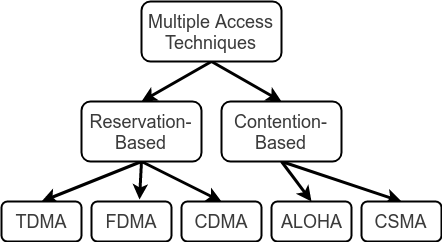
\includegraphics[width=0.5\textwidth]{pictures/mac_classification}
	\end{center}
	\caption{Classification of MAC techniques according to \cite{Garg07}}
\end{figure}

Traditional MAC protocols can be classified into one of two subgroups: reservation-based and contention-based. According to \cite{Bachir10} the appropriate choice of MAC protocol depends on a plethora of design-drivers such as requirements concerning throughput, latency, energy consumption and traffic patterns.

\subsection{Reservation-Based MAC Protocols}

Reservation-based protocols may implement an array of desirable features, but require knowledge of network topology in order to allow each node to communicate with every other on the basis of a schedule. These features include reduced collisions, fairness among nodes or multiple transmissions at the same time.

TDMA is a representative protocol in this group, which divides time into frames. Each frame is subdivided into slots, where each node is assigned to a unique slot during which it may transmit. As a result we obtain collision-free transmission, predictable scheduling delays, high throughput in heavy load situations and fairness among nodes. However, both the knowledge of topology and tight synchronization require large overheads or expensive hardware. As a result, TDMA becomes less attractive for large-scale networks \cite{Bachir10}.  


\subsection{ALOHA}
\label{sec:aloha}

ALOHA is arguably the most simple MAC protocol. Whenever a user wants to send data he just does so. The higher the channel load, i.e. sending requests per time unit, the more likely collisions will occur, which render all transmitted information useless.

The question is how likely it is that a collision does not occur. In other words, how efficient is an ALOHA channel? Making a statement requires a few preliminary assumptions as shown in \cite{Tanenbaum02}:

\smallskip

\begin{enumerate}
	\item We are taking a look at pure ALOHA.
	\item We simplify the calculation by assuming a fixed frame length.
	\item The number of packets generated during a frame time is a poisson-distributed random variable $X$.
	\item The channel load $G$ comprises of two portions: "new" and retransmitted frames.
\end{enumerate}



The probability mass function of the Poisson distribution and thus the probability of $k$ frames being generated during a given frame time amounts to:

\begin{equation}
	Pr(X=k) = \frac{G^k\cdot e^{-G}}{k!}
\end{equation}

The probability of zero frames being generated during the transmission of the frame is $Pr(X=0) = e^{-G}$ (assumption 3). If no collision occurs during the transmission of frame $F$ no other frame was sent off during that transmission. Conversely, $F$ itself did not collide with a frame sent off prior to $F$. We conclude that the vulnerability period during which collision may corrupt data is two frame times (assumption 2).

The probability that no frame other than the frame to be transmitted is generated during the two frame time vulnerability period is $P_0 = e^{-2G}$. The throughput $S$ is given by $S=GP_0 = Ge^{-2G}$.

The maximum throughput is achieved when $\frac{\partial S}{\partial G} \stackrel{!}{=} 0$:

\begin{eqnarray}
	& \frac{\partial S}{\partial G} & = \frac{\partial}{\partial G} Ge^{-2G} \\ 
	& & = e^{-2G}(1-2G) \\
	& & \stackrel{!}{=} 0 \\
	\Leftrightarrow & G & = 0.5
\end{eqnarray}
	
This means that for $G=0.5$ the throughput S reaches its maximum $S_\text{ALOHA,max} = \frac{1}{2e} \approx 0.18$. This result is very reasonable, since the transmission of a frame is vulnerable for the duration of two frame times, so the maximum is achieved when sending exactly every second slot, where a slot is equivalent to the frame time.

As an aside, the throughput can be doubled with slotted ALOHA. In contrast to pure ALOHA, slotted ALOHA allows transmission only at the beginning of slots, which effectively halves the vulnerability period to only one slot, since frames transmitted prior to a frame $F$ cannot interfere with $F$ anymore. Thus, $S_\text{ALOHA,max} = \frac{1}{e} \approx 0.36$, reached at $G=1$. However, this comes at the cost of an additional frame delay of $t_\text{slot}$ in the worst case and $\frac{t_\text{slot}}{2}$ in the average case and the need for synchronization. 

As shown in figure \ref{fig:aloha-csma-performance} ALOHA's performance is discouraging and improvements over ALOHA were found. 

\subsection{CSMA}
\label{sec:csma}

\begin{figure}[tb]
	\label{fig:aloha-csma-performance}
	\begin{center}
		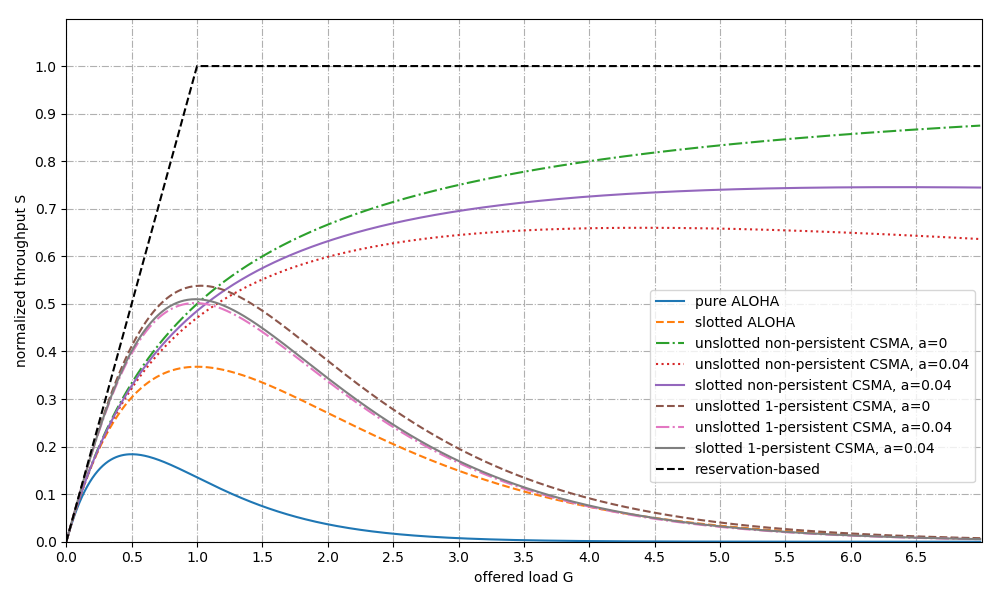
\includegraphics[width=\textwidth]{pictures/aloha_csma_performance}
	\end{center}
	\caption{Normalized throughput over offered load according to formulae in \cite{Garg07}, \cite{Bachir10},  \cite{Tanenbaum02}, with $a=\tau/T_p$, where $\tau$ is the maximum propagation delay and $T_p$ the packet transmission time and under the assumptions 2-4 made in section \ref{sec:aloha}. }
\end{figure}

Main problem of ALOHA is the negligence of concurrent traffic in the channel. A solution to this problem is offered by the "listen before talk" (LBT) mechanism, which means in order to avoid collisions we make a clear channel assessment (CCA) and refrain from sending should it be busy. This is the simple, yet effective basic idea of carrier sensing multiple access (CSMA) which comes in three flavors, as depicted in figure \ref{fig:csma-flavors} which will be discussed next.

\begin{figure}[tb] \label{fig:csma-flavors}
	\begin{center}
		\subfloat[1-persitent CSMA]{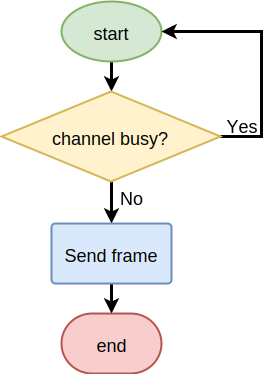
\includegraphics[width=0.22\textwidth,valign=c]{pictures/csma_1_persistent}}
		\qquad
		\subfloat[non-persistent CSMA]{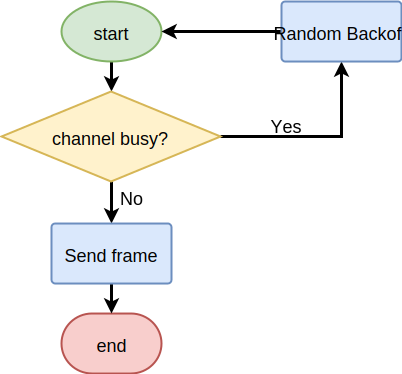
\includegraphics[width=0.31\textwidth,valign=c]{pictures/csma_non_persistent}}
		\qquad
		\subfloat[p-persistent CSMA]{\includegraphics[width=0.35\textwidth,valign=c]{pictures/csma_p_persistent}}
	\end{center}
\caption{The three flavors of CSMA}
\end{figure}


\subsubsection{1-Persistent CSMA}

When the channel is busy 1-persistent CSMA waits until the channel becomes idle. As soon as the channel is found idle a frame is transmitted with a probability of 1, hence 1-persistent CSMA. If the frame collides with another, the node waits for a random backoff time and then the whole process is started all over again.

Despite being a substantial improvement over ALOHA, this protocol has at least two problems:

\begin{itemize}
	\item Provided propagation delay is zero or negligible, collisions can still occur.  Imagine a three-node-scenario with nodes $A$, $B$ and $C$. $A$ is transmitting, while $B$ and $C$ are waiting for their turn. Once $A$ finished transmission $B$ and $C$ will lunge onto the channel like a pack of wolves leading to collision.
	
	\item If propagation delay is not negligible the protocol suffers from an additional problem. In this scenario $A$ has just begun sending. $B$ will assume the channel is idle and send off his frame, since, due to the propagation delay, $B$ has not yet heard of $A$. This is why propagation delay may significantly hamper this protocol's performance.
\end{itemize}  

\subsubsection{Non-Persistent CSMA}

In order to alleviate 1-persistent CSMA's problem with several nodes trying to seize the channel as soon as it becomes idle a less greedy attempt is made with non-persistent CSMA. Instead of continuously sensing the channel until it becomes idle nodes wait a random backoff time until they listen again. As a result, this protocol leads to better channel utilization with the downside of higher delays.

\subsubsection{P-Persistent CSMA}

P-persitent CSMA is a protocol for slotted channels. Whenever a node $A$ wishes to send off a packet the channel is sensed. If the channel is found idle it transmits its packet with a probability of $p$. With a probability $1-p$ it defers the transmissions to the next slot. This process is repeated until one either the packet is sent off or the channel is found busy again. In the latter case $A$ acts as though a collision had taken place and waits a random time until starting again.

This flavor of CSMA can be regarded as a compromise between 1-persistent CSMA and non-persistent CSMA, where the choice of $p$ determines the greediness. The smaller $p$, the less greedy and thus the closer p-persistent CSMA approximates non-persistent behavior. An appropriate choice of $p$ can get the best out of both worlds: minimal delays as in 1-persistent CSMA, as well as high channel efficiency as in non-persistent CSMA.

\subsection{CSMA with Collision Detection}

A way to further improve CSMA-family protocols is to immediately cancel transmissions once a collision is detected. There is no point in continuing these transmissions, as the transmitted data is lost in any case and aborting the transmission saves bandwidth, time and energy. 

CSMA/CD is used on wired LANs and serves as basis of the wide-spread Ethernet. However, this mechanism is not extensively made use of in wireless networks. Concerning the reason, it is cardinal to understand that collision detection is an analog process. A collision is detected by comparing the received and transmitted signal's energy or pulse width, which premises transmission and reception taking place simultaneously. This condition is seldom met for wireless nodes, which are mostly half-duplex. The reason for this lies in the conservation of energy, since wireless signal spreads spherically around its origin and thus degrades with the second order of distance. Furthermore, wireless channels are typically much more noisy than their wired counterparts and suffer from multipath fading. To make up for the loss in signal strength we would have to employ expensive signal processing in order to recover fainter signals. Alternatively, we could increase the transmit power, but this increases interference with other nodes, as well as electricity consumption.

%\begin{equation}
%	P = \int_{A} I(\vec{x}) \, dA
%\end{equation}
%
%Where $P$ is the power, $I$ the intensity as function of the position $\vec{x}$ and $dA$ the differential element of a closed surface around the source. Assuming that the integration takes place over the surface of a sphere with the radius $r$ the term simplifies to:
%
%\begin{eqnarray} 
%	& P = & \abs{I(r)} \cdot 4\pi r^2 \\
%	\label{eqn:intensity}
%	\Leftrightarrow & \abs{I(r)} = & \frac{P}{4\pi r^2} 
%\end{eqnarray}
%
%Another, and more common quantity in telecommunications is signal-to-noise ratio (SNR), which is defined as follows, where $P$ is the signal power and $N$ the noise power: 
%
%\begin{equation} \label{eqn:snr}
%	SNR [dB] = 10 \, log \left( \frac{P}{N} \right)
%\end{equation}
%
%Equations \ref{eqn:intensity} and \ref{eqn:snr} imply if we increase the distance $r$ by $\sqrt{2}$ the signal's intensity halves or lose 3dB in SNR, respectively. To make up for the loss in signal strength we would have to employ expensive signal processing in order to recover fainter signals. Alternatively, we could increase the transmit power, but this increases interference with other nodes, as well as electricity consumption.  

\subsection{Challenges for Wireless MAC Protocols}

Wireless MAC protocols have to tackle a few problems that do not occur in wired data exchange. Among them are the hidden node and the exposed node problem, which will be discussed by reference to \ref{fig:hidden_exposed_node_problem}. Further challenges, such as energy limitations will also be delineated.

\subsubsection{The Hidden Node and the Exposed Node Problem}

\begin{figure}[tb]
	\label{fig:hidden_exposed_node_problem}
	\begin{center}
		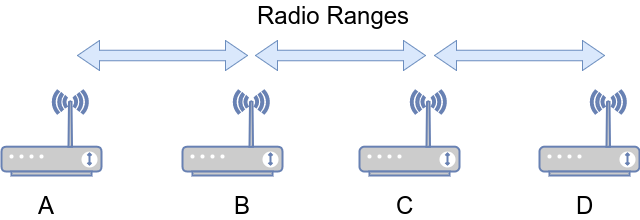
\includegraphics[width=12cm]{pictures/hidden_exposed_node_problem}
	\end{center}
	\caption{Setup to explain the hidden and exposed node problem. Each node can only reach its neighbors.}
\end{figure}

Suppose that the node's radio range is limited to the neighboring nodes and $A$ would like to transmit to $B$. If $C$ just started transmitting $A$ won't hear $C$ and falsely assume that the channel is idle and start transmitting. This is the hidden node problem.

For the same configuration, in another scenario $B$ would like to send to $A$ and $C$ is already transmitting to $D$. $B$ refrains from sending despite collisions would only take place between $B$ and $C$, where it does not matter. This is the exposed node problem. 

\subsubsection{Further Challenges}

% Citation needed for verification
Further challenges to MAC protocol design include the power conservation when faced with constrained power resources, as in wireless sensor networks (WSN) where devices rely on batteries for their supply with power. Attempts to mitigate waste of energy have been made in several specialized, duty-cycle based MACs such as Sensor MAC, Timeout MAC and Berkeley MAC as in more detail shown in section \ref{sec:duty-cycle-mac}.

On the same page, due to constrained energy resources, WSN are especially susceptible to denial of sleep attacks, a special form of denial of service (DoS) attack, drastically increasing energy consumption and thus reducing the system's lifetime. It is due to this fact that security is paramount in biomedical or military fields of application \cite{raymond09}. 

\subsection{CSMA with Collision Avoidance}

802.11 is a set of physical layer (PHY) and MAC specifications for wireless local area networks (WLANs). When the dominant mode of operation, the so-called distributed coordination function (DCF) is employed CSMA/CA is used in the MAC layer.

Beside physical carrier sensing previously simply referred to as carrier sensing another mechanism, namely virtual carrier sensing in combination with RTS/CTS exchange is (optionally) employed to mitigate the trouble caused by hidden nodes. 

In order to explain these mechanisms we refer to the setup of figure \ref{fig:hidden_exposed_node_problem} with a slight modification in so far as that each node's radio range shall span across two neighboring nodes in both directions. That is to say, $A$ can hear $B$ and $C$, but not $D$ and so on. Figure \ref{fig:virtual_carrier_sensing} visualizes the chain of events whose explanation follows.

\begin{figure}[tb]
	\label{fig:virtual_carrier_sensing}
	\begin{center}
		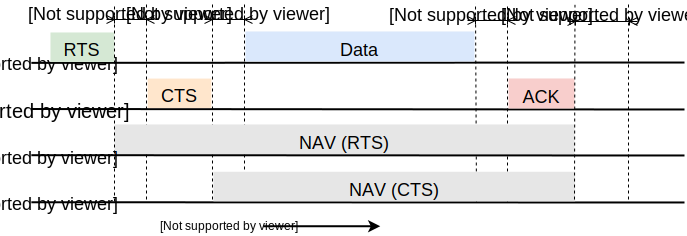
\includegraphics[width=14cm]{pictures/virtual_carrier_sensing}
	\end{center}
	\caption{Virtual carrier sensing in CSMA/CA, as described in \cite{Tanenbaum02} and \cite{Gast05}}
\end{figure}

$A$ wants to send to $B$, hence issues a request to send (RTS). Every node receiving the RTS is shut down, except for $B$ that in response to the RTS creates a clear to send (CTS) frame. Not only $A$ receives this CTS frame, but also $D$, a hidden node from $A$'s point of view. Upon reception of CTS $D$ is silenced as well. Therefore, RTS/CTS is addressing the hidden node problem. RTS/CTS are frames of 30 bytes length containing the length of the frame in this case $A$ wants to transmit. Based on this length $C$ and $D$ setup the so-called network allocation vector (NAV), which are node-internal timers reminding $C$ and $D$ that the channel is still in use. This mechanism is called virtual carrier sensing due to the fact that no physical process is involved in obtaining the channel status. Shutting down nodes has the beneficial side-effect of reducing overhearing and therefore reduces energy consumption.

As further depicted in figure \ref{fig:virtual_carrier_sensing} there are named intervals of specified length between each of the frames. Varying lengths of these interval types serve the purpose of prioritizing certain frames over others. 

The short interframe spacing (SIFS) is the interval until the next control frame or next fragment (of a fragmented data frame) may be sent. SIFS is designed to allow one party out of the two parties in dialog send off their frame without interference by another node. The longer interval DCF interframe spacing (DIFS) is the interval after which any station may try to seize the channel for their transmission.

For the sake of completeness, we briefly mention two previously consciously left out intervals, namely point coordination function interframe spacing (PIFS) and extended interframe spacing (EIFS). If 802.11 is operates in an alternative mode of operation, where the base station acts as point coordinator of traffic the standard prescribes an interval of length PIFS to allow the base station to send certain control (beacon and poll) frames. EIFS is used to report the reception of a bad or unknown frame and due to this action's low priority is the longest interval among the mentioned four. 

\subsection{Duty-Cycle-Based MAC Protocols} \label{sec:duty-cycle-mac}  

In duty-cycle-based MAC schemes nodes repeatedly alternate between active and sleep phases to reduce idle listening and thus energy consumption. Due to increased contention during active phases these protocols are mostly designed for limited contention traffic situations as in WSNs. The share of an active period in a cycle is called duty factor. Sources to this section were \cite{Bachir10} and \cite{Demirkol06}.

\subsubsection{Sensor MAC}

In SMAC the active period is divided into to a synchronization and a data transmission phase. During sync phase nodes transmit SYNC packets. Nodes receiving SYNC packets adopt the schedule carried by the packet and broadcast into their neighborhood. Nodes that follow the same schedule form a virtual cluster. Borderline nodes between virtual clusters adopt multiple schedules and thus have an increased duty factor. During contention period SMAC features the RTS/CTS exchange and fragments data frames, which are transmitted in a burst to reduce collision likelihood. The duty factor per schedule is predetermined on the basis of expected load as the result of an optimization problem on the competing goals of reducing idle listening and contention. The higher the duty factor the more idle-listening and the less contention occurs.

\subsubsection{Timeout MAC}

While TMAC shares the same principle of schedule establishment with SMAC nodes adaptively vary duty factors depending on expected traffic. Furthermore, TMAC shifts all communication to the beginning of the active period. This allows nodes to sleep earlier should no traffic be detected during a certain time period. In variable load situations TMAC saves as much as five times more energy compared to SMAC at the cost of increased latency. 

\subsubsection{Berekeley MAC}

Still, TMAC maintains common active phases at high energy expenses. BMAC drops the requirement of maintaining common active phases. Instead payload is preceded by extended preambles such that every receiver is able to reliably detect packets. This has the effect of shifting energy expenses from the receiving to the sending side, which saves energy in low load applications such as surveillance. In BMAC CCA is based on outlier detection, instead of thresholding like in CSMA further reducing energy use \cite{Polastre04}. 

\subsection{LTE in the Unlicensed Band}
\label{sec:lte-mac}

The base station (eNB) of LTE in the licensed band coordinates traffic by assigning physical resource blocks (PRB) to users. The set of PRBs is a cartesian product of frequency and time slots based on the reservation techniques of OFDMA and TDMA. 

Clearly, additional measures need to be taken if LTE was to share the unlicensed bands with contention-based services such as WiFi. The two principal approaches to ensure harmonious coexistence of LTE and WiFi in the unlicensed band are on the hand LTE-U, a duty-cycle-based approach (LTE-U CSAT) and on the other hand LAA, relying on LBT. Since LAA in large part resembles CSMA/CA's LBT mechanism it seems quite natural to assume it will coexist better with WiFi \cite{kwon17}.

With the carrier aggregation (CA) in LTE Unlicensed primary cells (PCells) used to establish and maintain the connection of UE (user equipment) to the network and secondary cells (SCells) need to be distinguished. One or more additional SCells can be allocated to extend a UE's bandwidth. On the grounds that the unlicensed carrier is shared with multiple systems the same QoS, reliability and mobility cannot be achieved as on the licensed carrier. For this reason unlicensed carriers are only considered to be supplemental downlink (SDL) SCells.

\section{Software Defined Radio}
 
\subsection{Purpose of Software Defined Radio}

Traditional radio equipment is "hardware-defined", i.e. that the signal processing runs on a specialized electrical circuit. This has the potential advantages of efficient energy use and cheap production at the cost of limited flexibility in operation. 

In SDR signal processing components such as filters, amplifiers, modulators, detectors and many more are implemented in software and mostly run on general-purpose processors, sometimes in combination with DSPs and FPGAs.

While the limitations of hardware-defined radios are acceptable for a number of applications, such as e.g. self-made radio receivers as shown in figure \ref{fig:radio-receiver-circuits}, it is very desirable to get rid of these limitations for rapid prototyping of new technologies including but not limited to cognitive radio, software-defined antennas and wireless mesh networks. In the case of this thesis SDR simplifies studying the influence of different MAC mechanisms.

\begin{figure}[t]
	\label{fig:radio-receiver-circuits}
	% source: http://electronicsforu.com/electronics-projects/simple-fm-receiver 03.10.17
	% source: http://www.electroschematics.com/9043/am-receiver-circuit/ 03.10.17
	\begin{center}
		\subfloat[FM Receiver]{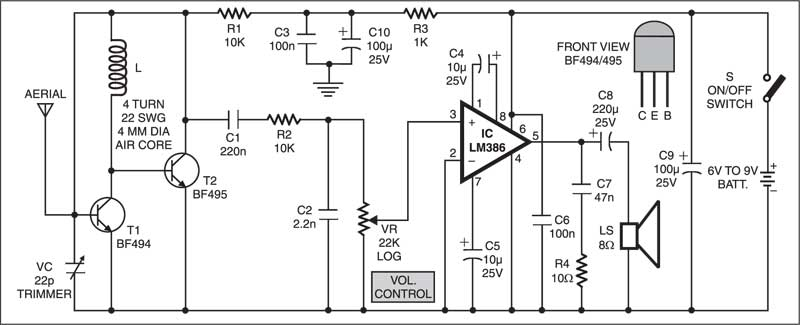
\includegraphics[width=0.5\textwidth,valign=c]{pictures/fm_radio_receiver_circuit}}
		\qquad
		\subfloat[AM Receiver]{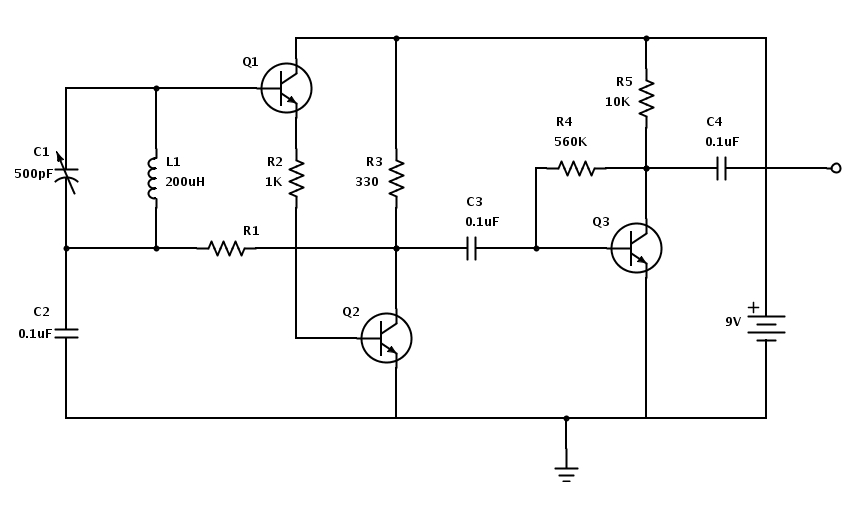
\includegraphics[width=0.4\textwidth,valign=c]{pictures/am_radio_receiver_circuit}}
	\end{center}
	\caption{Simple DIY radio receiver circuit diagrams}
\end{figure}

\subsection{What is GNU Radio?}

\label{sec:gnu-radio}

The GNU Radio (GR) project is dedicated to the evolution of a free and open-source SDK enabling both the creation of actual software-defined radio, as well as simulated signal processing. Written in C++ and Python, GNU Radio also comes with the intuitive graphical software GNU Radio Companion (GRC) that allows creating block diagrams called flowgraphs simply by connecting signal processing blocks into a directed graph. Its audience is not merely limited to research and industry, but also encompasses academia, government and private users.

A proprietary, well-documented alternative to GNU Radio is LabVIEW developed by National Instruments. LabVIEW takes a purely graphical approach similar to GRC relying on block diagrams, but lacks the freedom of user-defined block creation with a programming language such as C++ or Python.

Mathworks MATLAB/Simulink also provides a communication systems toolbox, however the institute's devices are not on the list of officially supported devices \cite{Matlab}.

\begin{figure}[t]
	\label{fig:gnuradio}
	% source: http://electronicsforu.com/electronics-projects/simple-fm-receiver 03.10.17
	% source: http://www.electroschematics.com/9043/am-receiver-circuit/ 03.10.17
	\begin{center}
		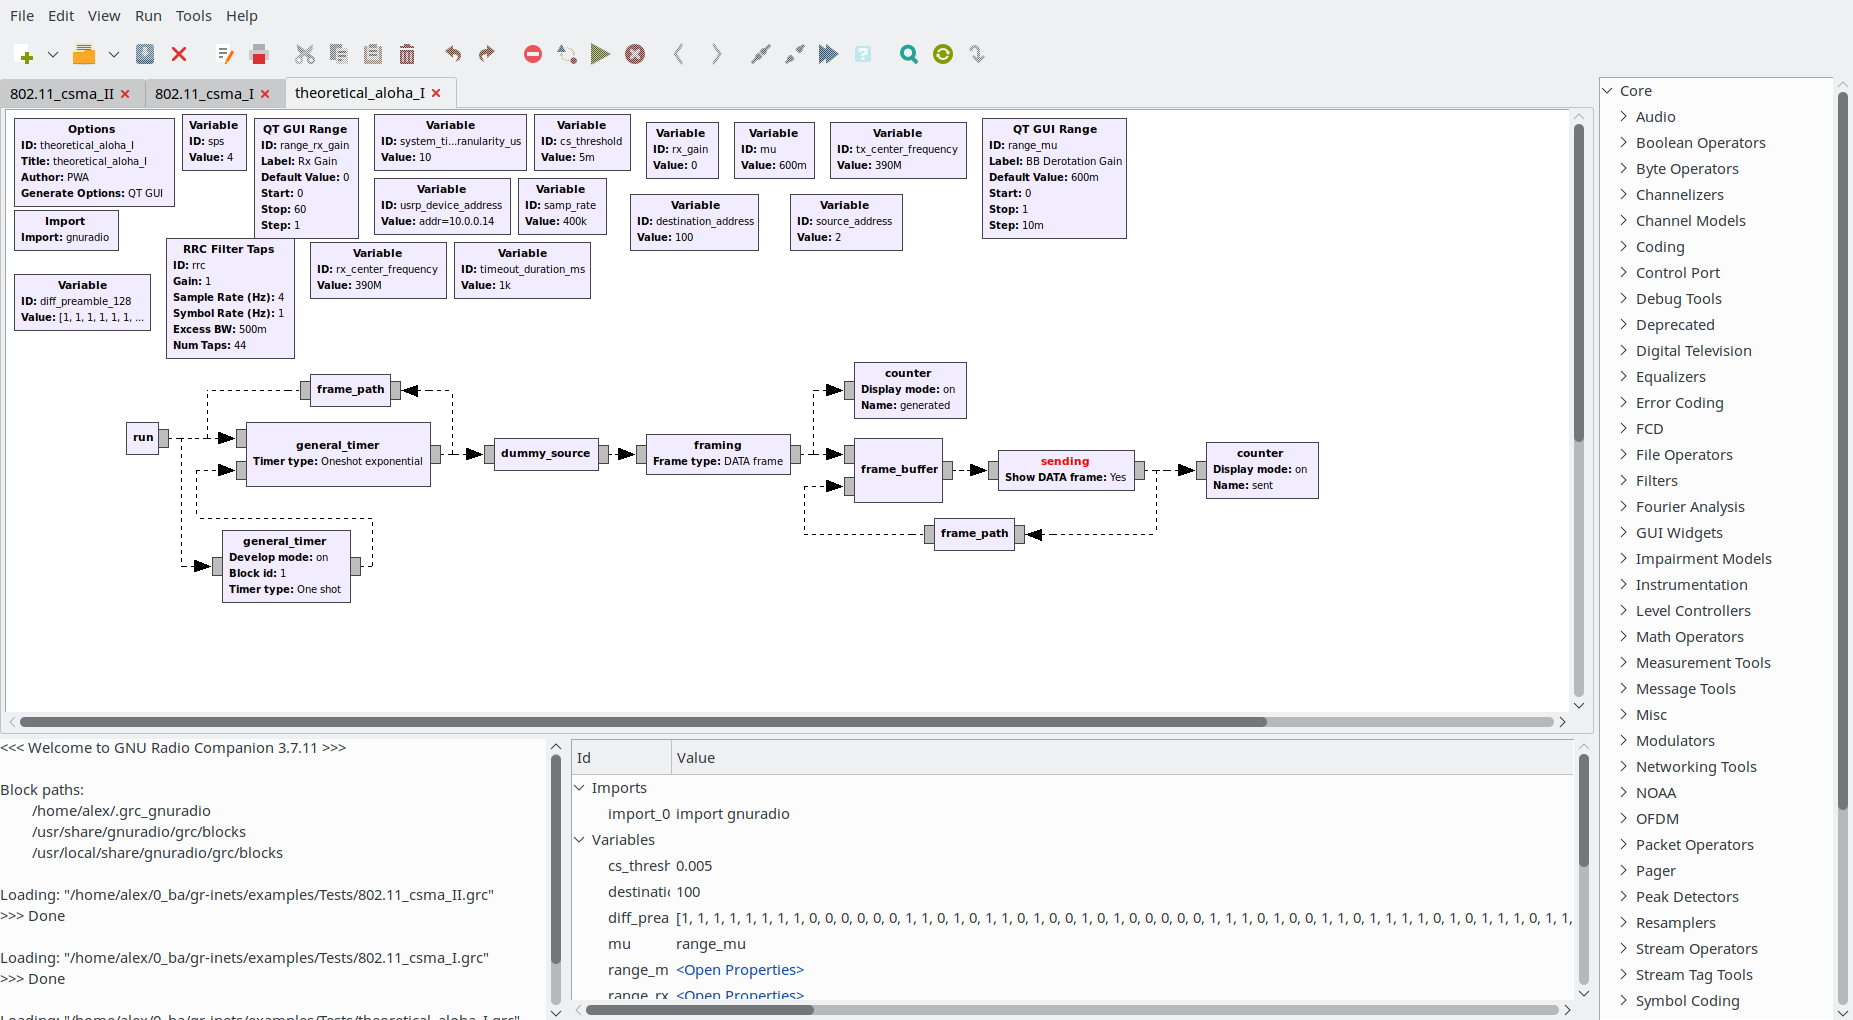
\includegraphics[width=0.9\textwidth,valign=c]{pictures/grc_ui}
	\end{center}
	\caption{GNU Radio Companion GUI}
\end{figure}

\subsection{Core Concepts of GNU Radio}

\subsubsection{Flowcharts and Blocks}

The two most basic concepts of GNU Radio are flowgraphs and blocks. As mentioned in \ref{sec:gnu-radio} flowgraphs are directed graphs, whose nodes are functional blocks and whose vertices determine the direction of data flow \cite{GR1}. 

The behavior of these blocks is programmed in either Python or C++, where the latter is recommended for performance-critical applications, which is also why the blocks in our flowgraphs are all written in C++. If performance is less critical Python is a superior choice since it is more concise and allows faster prototyping as there is no need for compilation. Each block generally serves exactly one purpose for the sake of modularity. Blocks in turn can be composed of an arbitrary number of inner blocks, making extensive use of the modularity and hiding implementation complexity from the user, much like a blackbox in electrical circuits. These composed blocks are called hierarchical blocks. In our case the complete PHY layer is hidden in hierarchical blocks called "sending" and "receiving".

Blocks are connected through ports, which can either be input or output ports. Depending on which types of ports a block has, it can either be a source, sink or neither of the former. 
Each input port only consumes data of a specific data type. Similarly, each output port only produces data of a specific data type. The set of types ranges from integers, floating point and complex numbers to messages and a bunch of others. Since each block implements a certain function these ports can be regarded as input parameters and return values of a function, respectively.

\subsubsection{Message Passing and Stream Tags}

When designing packet-based protocols, such as MAC protocols it is of tremendous importance to be able to detect packet data unit (PDU) boundaries. For this purpose GR provides an asynchronous message passing system. A synchronous alternative is to attach so-called stream tags to the "infinite" stream of data. The former method is the right choice when designing MAC protocols due to the asynchronous nature of packet delivery \cite{GR1}\cite{GRDocs}.  

\subsubsection{Polymorphic Types and SWIG} 

Polymorphic types (PMT) are opaque data types that enable safe information exchange across blocks by serving as generic containers of data. Self-evidently, the original data type must be retained as a PMT class member. For thread-safety reasons PMT are immutable. We make extensive use of PMTs when passing messages. As an aside, note that the python PMT class has some powerful tools unavailable its C++ counterpart, making use of Python's weak typing \cite{GRDocs}.

SWIG (simplified wrapper and interface generator) is a software that helps to connect code written in C or C++ to a variety of scripting languages, such as in our case Python. This is achieved by generating a Python module from the C/C++ code with the help of an interface file. This "compatibility layer" is necessary, because blocks can be written in either Python or C++ as mentioned earlier.
\chapter{Related Work}
\label{ch:related-work}

This chapter introduces work related to the thesis. We will highlight similarities and differences of various studies to our work. 

In the following section we discuss approaches and results of studies that examined the coexistence of different technologies in the same frequency band. Studies concerning inter-technology coexistence are based on at least one of the following: theoretical analysis, simulation or measurements with physical devices. Due to the fact, that we also carry out experimental research using USRPs, we are more interested in studies based on the latter. Furthermore, studies based on measurement with real devices have the benefit of better reflecting system level details of the technologies and providing insight for real-world deployments. However, as pointed out in \cite{gomezmiguelez16} vendor-specific properties of the test hardware must be taken into account since they may exert great influence on the measurement results. Some studies propose new mechanisms for one of the technologies which we do not do.

\paragraph{LTE-U/Wi-Fi Coexistence}
Although a great number of simulation-based studies \cite{nihtilä13}, \cite{rupasinghe14}, \cite{jeon14}, \cite{cavalcante13} exist on this topic we will confine the discussion to two studies \cite{gomezmiguelez16}, \cite{capretti16} based on measurements with physical devices. Both studies evaluate LTE Unlicensed /Wi-Fi coexistence based on LTE-U using srsLTE, an open-source SDR library to implement the PHY layer of LTE. Another common feature of both studies is the use of USRPs as LTE nodes. 

In \cite{gomezmiguelez16} the testbed comprises of several Wi-Fi and LTE links, for which they used Ettus USRP B210 boards (LTE) and low-power single-board computers from Soekris (Wi-Fi). In order to detect vendor-specific performance issues they decided to use two different sets of wireless NICs from Atheros and Broadcomm. In their study the influence of the following parameters was examined: LTE-U duty cycle, Wi-Fi and LTE TX power, LTE bandwidth, LTE central frequency (i.e. LTE and Wi-Fi spectrum overlap). Their main results can be summarized as follows:
\begin{itemize}
	\item  Wi-Fi throughput is inversely proportional to LTE duty cycle.
	\item  Wi-Fi TX power has little impact on Wi-Fi throughput.
	\item  The influence of LTE bandwidth and central frequency on Wi-Fi throughput depends very much on the vendor of the NIC card. As a consequence, more experimental research with physical devices from different vendors is strongly recommended. 
\end{itemize}
  
The testbed in\cite{capretti16} consists of one LTE base station (eNodeB or eNB) and one user equipment (UE), one Wi-Fi access point and five other Wi-Fi nodes. Their Wi-Fi network was based on embedded PCs equipped with commodity wireless adapters. The LTE nodes were based on desktop computers with Ettus USRP B210 RF front ends running the open-source driver UHD. An interesting detail is that they also used GNU Radio. The following parameters were subject of interest: duty cycle, Wi-Fi power settings Wi-Fi MCS (modulation and coding scheme) and packet size. The metrics measured were satisfied load in percent, total Wi-Fi throughput, Wi-Fi jitter and LTE packet loss.  Their main findings can be summarized as follows: 
\begin{itemize}
	\item The duty cycle patterns are a main influence on achievable Wi-Fi throughput. Particularly, shorter duty cycles decrease jitter, which is important for real-time applications. On the other hand longer duty cycles offer superior throughput due to reduced overhead.
	\item LTE suppresses Wi-Fi transmissions if the TX power levels are comparable and no duty cycling is employed.
	\item If Wi-Fi TX power is increased, Wi-Fi load negatively impacts LTE throughput. There is no panacea strategy ensuring maximum Wi-Fi throughput operating under different MCSs and packet sizes. LTE performance is unaffected by Wi-Fi contention levels.
\end{itemize}

Both studies are similar to our work in so far that they use SDR with real hardware to experimentally evaluate inter-technology coexistence. However, the examined parameters of their studies are mostly related to power, frequency and duty-cycle, whereas we focus on CSMA/CA timing aspects.

\paragraph{ZigBee/Wi-Fi Coexistence}

In the MAC layer ZigBee uses the CSMA/CA protocol in nonbeacon-enabled mode or a mixture of CSMA/CA and TDMA in beacon-enabled mode. If upper layers detect that the throughput degrades below a certain threshold the MAC layer will be instructed to perform an energy scan through all available channels after which follows a switch to the channel with the lowest detected energy \cite{yi11},\cite{zhang11}. 
The comprehensive study \cite{yi11}, which is based on theoretical analysis, simulation (using Matlab/Simulink) and measurement with real devices take an approach that differs from ours. Instead of relying on the CSMA/CA algorithm in contention situations they try to avoid sharing the same channel with Wi-Fi. They conclude that adhering to certain deployment rules or alternatively appropriate channel management guarantee good coexistence of Wi-Fi and ZigBee:
\begin{itemize}
	\item A frequency offset of 8 MHz between the Wi-Fi and ZigBee channel central frequencies with a distance of 2 m between Wi-Fi and ZigBee nodes is always sufficient. In such a case adjacent channel interference is negligible.
	\item Alternatively a distance of 8 m between Wi-Fi and ZigBee nodes is always sufficient.
	\item If the former two rules are not applicable smart channel management can drastically reduce interference with Wi-Fi.
\end{itemize}

In \cite{zhang11} a SDR testbed with USRPs and GNU Radio is deployed to evaluate the influence of a proposed mechanism, namely cooperative busy tone, on the throughput of ZigBee and Wi-Fi. The idea is that a separate ZigBee node schedules a busy tone whenever a transmission between nodes is desired to enhance the visibility of ZigBee to Wi-Fi nodes. 

The ZigBee Alliance white paper \cite{thonet08} shows that ZigBee can coexist well with Wi-Fi in home networks if the Wi-Fi load is low. However, as Wi-Fi load increases to medium and high loads ZigBee throughput decreases severely in \cite{gummadi09} and \cite{polin08}. All three of these papers are based on measurements with physical devices, but none features SDR. Furthermore, the focus in these papers lies on different traffic patterns, a subject we only touch.

\paragraph{Bluetooth/Wi-Fi Coexistence}
Bluetooth is a coordination-based technology where a master device and up to seven active slave devices form a piconet using adaptive frequency hopping, which is a type of frequency hopping spread spectrum, which is a CDMA technique. With the pseudo-random frequency hopping scheme Bluetooth may interfere with Wi-Fi nodes. The simulation-based study \cite{chiasserini02}, in contrast to our work, proposes two algorithms to avoid overlapping of Bluetooth with Wi-Fi in the time and the frequency domain, respectively, rather than evaluating the influence of parameter variation on standardized mechanisms. The key idea of the first algorithm is to adjust the Wi-Fi packet length to fit in between two Bluetooth packet transmissions. The second algorithm induces the Bluetooth master node to schedule data packets with appropriate durations to skip the frequencies of the hopping pattern that are expected to drop on the IEEE 802.11 band. The similarities of this study to our work is limited to examining coexistence mechanisms.
\chapter{Measurement Methodology}
\label{ch:methodology}

This chapter describes methods and scenarios of the measurements we have taken. Firstly, the measurement testbed is discussed. Secondly, we define central terms to guard against misapprehensions. Thereafter, we give an overview of the MAC protocols we empirically evaluated, implemented as GNU Radio flowgraphs. Subsequently, measurement metrics which we use in chapter \ref{ch:results} to analyze the performance of the protocols are formally defined with reference to the flowgraphs. Thereafter, an overview of the semi-automatic measurement script system designed to automate, therefore accelerate the process of file system management, data processing and result plotting is given. Eventually, we discuss the quality norms of the measurements.

\section{Measurement Testbed}

The setup consists of two USRP2s from Ettus Research and two USRP 2920s from National Instruments. The first two USRPs are programmed as receiver and sniffer, respectively, whereas the latter two as transmitters, as depicted in \ref{fig:measurement-setup}. Each USRP was connected to a gigabit switch through a LAN cable. The scripts running on the devices were launched from a local computer with the IP 134.130.223.151, which was remotely controlled from a laptop. Both transmitters sent their data to the single receiver. Hereafter, we will call the node pair 10.0.0.9-10.0.0.6 link 1 and 10.0.0.3-10.0.0.6 link 2. Tables \ref{tab:measurement-parameters} and \ref{tab:measurement-parameters-2}  contains other necessary configuration parameters to reproduce the measurement results.

\begin{figure}[tb]
	\label{fig:measurement-setup}
	\begin{center}
		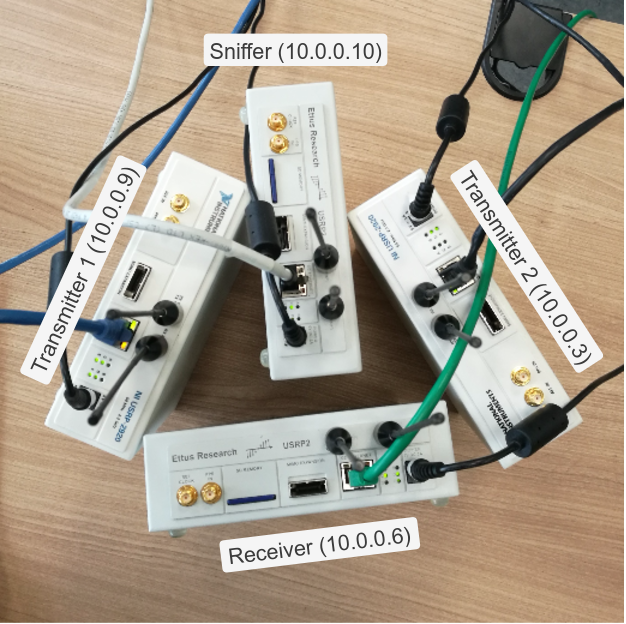
\includegraphics[width=0.5\textwidth]{pictures/measurement_setup}
	\end{center}
	\caption{Photo of the measurement setup. The transmitters 10.0.0.3 and 10.0.0.9 transmit their data to the receiver 10.0.0.6. Their conversations are overheard by the sniffer 10.0.0.10.}
\end{figure}

% Measurement parameters
\begin{table}[t]
	\label{tab:measurement-parameters}
	\begin{center}
		\begin{tabular}{*{14}{|c}|}
			\hline
			Function & TX Gain & RX Gain & Source Address & Dest. Address & IP Address\\
			\hline
			Receiver 		& 4 dB 	& 10 dB & X 	& any	& 10.0.0.6\\
			Sniffer 		& 0 	& 0 	& any 	& any	& 10.0.0.10 \\
			Transmitter 1 	& 5 dB 	& 0 	& Y 	& 	X 	& 10.0.0.9 \\
			Transmitter 2	& 9 dB 	& 0 	& Z 	& 	X 	& 10.0.0.3 \\
			\hline	
		\end{tabular}\caption{Device-specific setup parameters.}
	\end{center}
\end{table}

\begin{table}[t]
	\label{tab:measurement-parameters-2}
	\begin{center}
		\begin{tabular}{*{14}{|c}|}
			\hline
			Layer & Parameter & Value & Comment\\
			\hline
			 			& MCS & QPSK & BPSK optional, unused\\
			PHY Layer	& Central frequency & 450 MHz & 420 MHz - 480 MHz work as well \\
						& Sampling rate & 400k/s & \\
			\hline	
						& Frame size & 1000 bytes & max. supported by OS\\
						& Payload size & 837 bytes & \\
			MAC Layer	& Timeout & 100 ms & $\text{RTT \le 68 ms}$ \\
						& CSMA CS threshold & 0.001 PU & for RX/TX gains as in Table \ref{tab:measurement-parameters} \\  
						& Max. retransmissions & 6 & \\
			\hline	
		\end{tabular}\caption{General setup parameters.}
	\end{center}
\end{table}

\section{Measurement Protocols and Scenarios}
\label{sec:measurement-scenarios}

Next, we define some central terms used throughout the remainder of the thesis and then present the measurement scenarios.

\paragraph{Traffic Saturation}
If not specified otherwise all transmitters are backlogged, i.e. we have \emph{saturated} traffic. In that case the time between the generation of each packet is constant and well below the RTT. When we use the term \emph{unsaturated} the time between packets generated by the \code{dummy\_source} is exponentially distributed with $\frac{1}{\lambda}=200ms$. These packets are then buffered in a \code{frame\_buffer}. For single link scenarios this leads to Poisson-distributed traffic.

\paragraph{Measurement and Repetition}
In this thesis \emph{measurement} refers to a period of 500 seconds comprising of five \emph{repetitions} with a duration of 100 seconds each. 

\paragraph{Baseline and Coexistence Measurements}
When referring to the term \emph{baseline} measurement we mean that only one of the two links was active. If both links were active we refer to a \emph{coexistence} measurement. The baseline measurements serve two purposes: confirming that the devices work properly and for comparison with the coexistence measurements. A more detailed description on baseline measurements can be found in Section \ref{sec:quality-standards}.   

\paragraph{Measurement Scenarios}
A scenario is a combination of  MAC protocols employed on the two links as depicted in Table \ref{tab:measurement-scenarios}. We distinguish between two types of scenarios. In "same MAC" scenarios the same MAC protocol is employed on both transmitters. In "different MAC" scenarios different MAC protocols are employed on the transmitters.

\paragraph{Pure ALOHA}
We implement the pure ALOHA protocol based on the theory in Section \ref{sec:aloha} as GNU Radio flowgraph depicted in Figure \ref{fig:grc-aloha-transmitter} and described in Section \ref{sec:aloha-transmitter}.

\paragraph{CSMA/CA}
We implement CSMA/CA based on the theory in Section \ref{sec:csma-ca}. The flowgraph is depicted in Figure \ref{fig:grc-csma-transmitter} with the corresponding description found in Section \ref{sec:csma-transmiter}. We are \textbf{not} featuring the optional IEEE 802.11 RTS/CTS exchange, realize DIFS and SIFS with \code{general\_timers} and the backoff with the \code{backoff} blocks. In two of three measurement variants we set SIFS, DIFS and backoff slot (BO) times to different scaled versions of their values\footnote{The values of DIFS, SIFS and BO in the IEEE 802.11g standard are $\text{DIFS}=50 \,\text{\mu s}$, $\text{SIFS}=10 \,\text{\mu s}$, $\text{BO}=20 \,\text{\mu s}$, $\text{CW}_\text{min}=31$,  $\text{CW}_\text{max}=1023$ \cite{802.11g}.} prescribed in the IEEE 802.11g standard. We refer to these two variants as the high parameter values ($\text{DIFS}=15\,\text{ms}$, $\text{SIFS}=3\,\text{ms}$, $\text{BO}=6\,\text{ms}$) and the low parameter values ($\text{DIFS}=5\,\text{ms}$, $\text{SIFS}=1\,\text{ms}$, $\text{BO}=2\,\text{ms}$). The third variant are the medium parameter values based on the low parameter set but with $\text{DIFS}=9\,\text{ms}$. We employ the same $\text{CW}_\text{min}=31$ and $\text{CW}_\text{max}=1024$ as the IEEE 802.11g standard.

\paragraph{1-persistent CSMA}
For 1-persistent CSMA we use the same flowgraph as for CSMA/CA and set SIFS and backoff slot times to zero. In contrast to theoretical p-persistent CSMA we sense the channel for DIFS instead of a minimal number of samples. More accurately, we could describe the protocol as "1-persistent CSMA-like with fixed sensing duration", but for brevity's sake we will refer to it as 1-persistent CSMA.  
 
\begin{table}[bt]
	\label{tab:measurement-scenarios}
	\begin{center}	
		\begin{tabular}{*{14}{|c}|}
			\hline
				 Scenario Type & Link 1 & Link 2 \\
			\hline
				 & \multicolumn{2}{c|}{ALOHA} \\ 
				Same MAC & \multicolumn{2}{c|}{CSMA/CA (3 variants)} \\
				& \multicolumn{2}{c|}{1-persistent CSMA} \\ 
				\hline
				& ALOHA & CSMA/CA \\
				& unsaturated ALOHA & CSMA/CA \\
				Different MAC & CSMA/CA & CSMA/CA \\
				& 1-persitent CSMA & unsaturated ALOHA \\
				& 1-persistent CSMA & CSMA/CA \\
			\hline
		\end{tabular}\caption{Measurement Scenarios.}
	\end{center}
\end{table}

\section{GNU Radio Flowgraphs}    

A GNU Radio flowgraph is a directed graph, each of whose vertices called blocks implements a certain functionality of the MAC protocol. The edges determine the direction of data flow as discussed in Section \ref{sec:flowgraphs}.

\subsection{Receiver and Sniffer}

%frame_analysis block missing
Figure \ref{fig:grc-receiver} shows the two-way handshake receiving logic. After frame integrity is checked by the \code{frame\_check} block and the type is confirmed to be data frame an acknowledgment is generated by the \code{frame\_type\_check} block. The \code{frame\_probe} blocks record the times when the frames reach certain positions in the flowgraph representing the occurrence of events such as frame reception, passed or failed frame integrity check and more. Note that the address check is disabled so that the receiver may receive frames from any transmitter.

The sniffer (flowgraph in Figure \ref{fig:grc-sniffer}) consists only of a single \code{frame\_probe} block, which records detected power above noise level during the whole measurement. The sniffer provides valuable insight of what is actually going on in the channel from a "neutral" point of view - neutral in the sense of:

\begin{itemize}
	\item A clear distinction between the transmitters can be made according to the received energy levels, since the sniffer is located between the transmitters and transmission gains were chosen accordingly.
	\item Sensing the channel is possible during the whole measurement time, because the sniffer is never sending.
\end{itemize}

In a nutshell, the sniffer is a valuable debugging and verification tool as described in more detail in section \ref{sec:measurement-metrics}.

\begin{sidewaysfigure}[ht]
	\begin{center}
		\subfloat[Receiver]{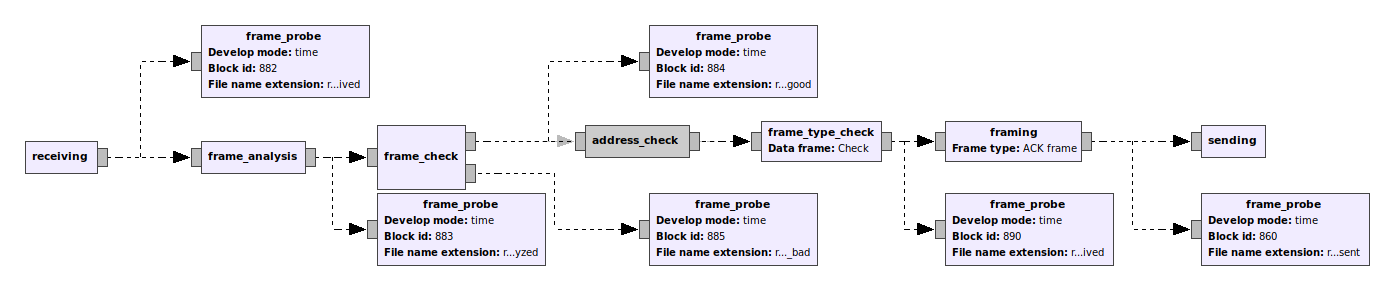
\includegraphics[width=\textwidth]{pictures/grc_receiver_flowgraph}}
		\label{fig:grc-receiver}
		\vskip 40pt
		\subfloat[Sniffer]{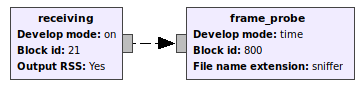
\includegraphics[width=0.3\textwidth]{pictures/grc_sniffer_flowgraph}}
		\label{fig:grc-sniffer}
	\end{center}
	\caption{GRC Receiver Flowgraphs.}
\end{sidewaysfigure}

\subsection{Pure ALOHA Transmitter}
\label{sec:aloha-transmitter}

The flowgraph, whose discussion follows, is depicted in Figure \ref{fig:grc-aloha-transmitter}. The \code{run} block enables us to start several transmitters exactly at the same time, which is useful if we execute the flowgraphs manually without the automated measurement scripts. Payload is generated in the \code{dummy\_source} block, packed into a frame in the \code{framing} block and buffered in the \code{frame\_buffer} block. The interval between generated frames is determined by a \code{general\_timer} block, which we trigger either in constant or exponentially distributed intervals. Self-reception is prevented by shutting down the receiver when about to send a frame through the sending block. As soon as the data packet is sent off the \code{timeout} block receives a copy of the data frame. If the timeout timer is reset by a recevied ACK before it runs out the next frame in the buffer is dequeued, otherwise the data is forwarded to the \code{resend\_check} block. If the maximum number of retransmissions, in our case 6 has not been reached a retransmission is issued, otherwise the frame is dropped without substitution.

\begin{sidewaysfigure}[h]
	\label{fig:grc-aloha-transmitter}
	\begin{center}
		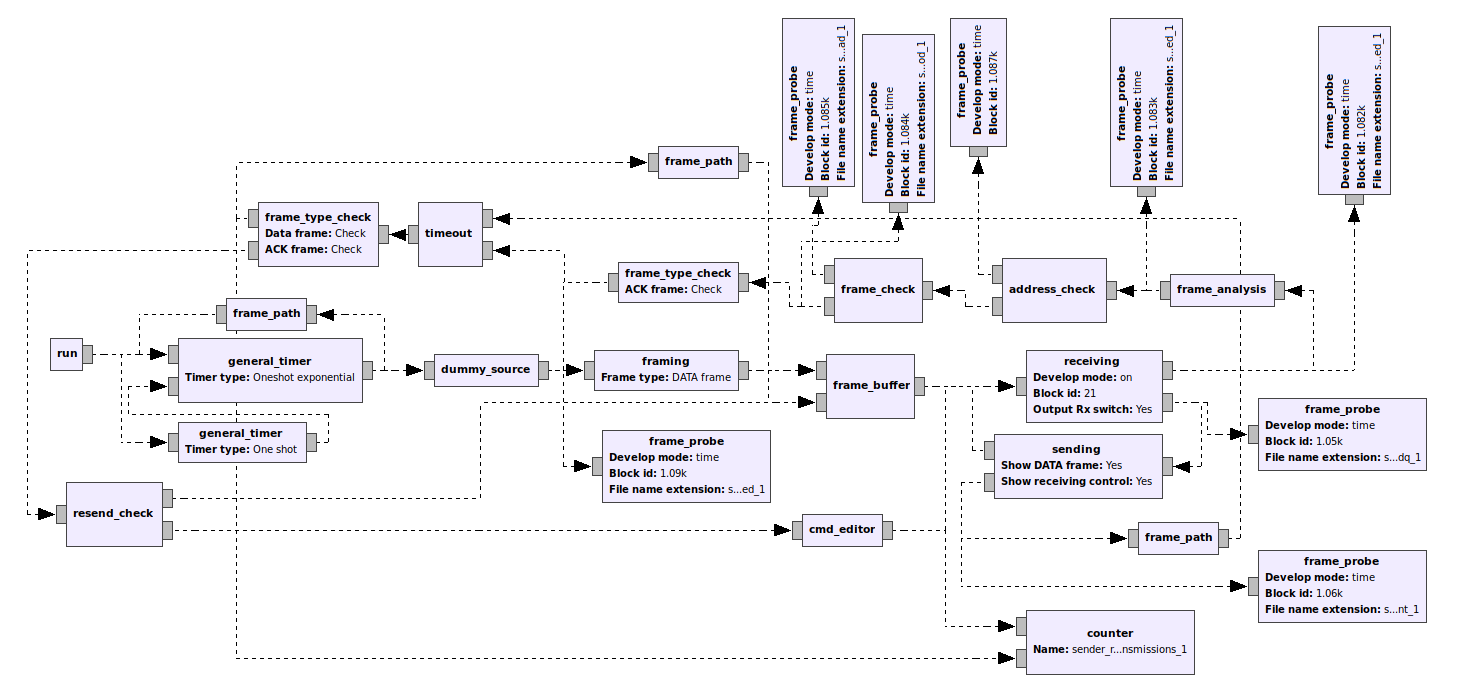
\includegraphics[width=\textwidth]{pictures/grc_aloha_transmitter_flowgraph}
\end{center}
\caption{GRC Pure ALOHA Transmitter Flowgraph.}
\end{sidewaysfigure}

\subsection{CSMA Transmitter}
\label{sec:csma-transmiter}

The CSMA transmitter (Figure \ref{fig:grc-csma-transmitter}) is based on the ALOHA transmitter, but features extra mechanisms as described in section \ref{sec:csma}, which will now be discussed. The flowgraph aims at resembling IEEE 802.11 DCF and features CCA through thresholding in the \code{carrier\_sensing} block. Despite the fact that this block has the feature of adaptively determining an appropriate carrier sensing threshold we chose a fixed value of 0.002 power units (PU) \footnote{Power unit is a linear-scale unit read out via the UHD driver.}. This choice was made to make sure that ALOHA transmission power levels were not confused with noise during the adaptive CSMA noise floor detection period. 

DIFS and SIFS are realized through \code{general\_timer} blocks with the respective values. The design, as depicted, does not feature the RTS/CTS exhange.

\begin{sidewaysfigure}[h]
	\label{fig:grc-csma-transmitter}
	\begin{center}
		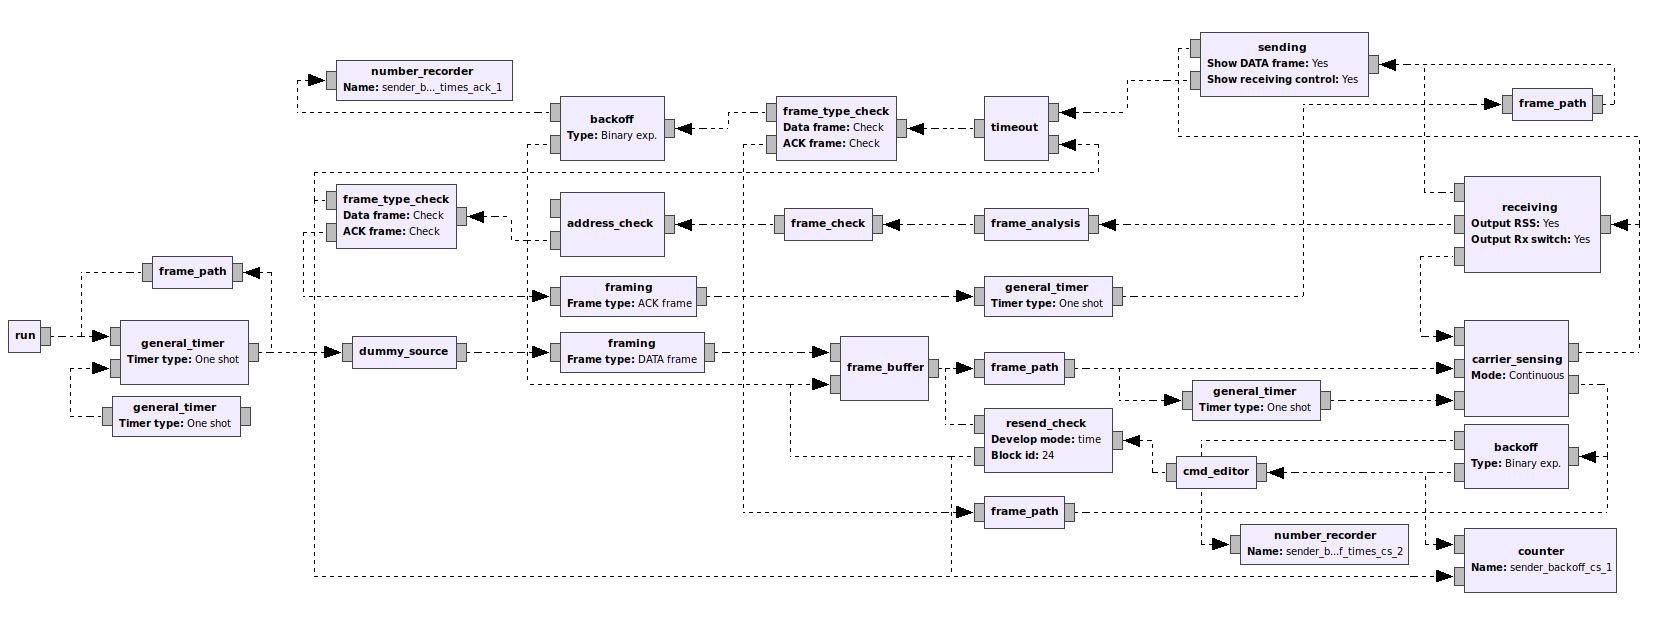
\includegraphics[width=\textwidth]{pictures/grc_csma_transmitter_flowgraph}
\end{center}
\caption{GRC CSMA Transmitter Flowgraph.}
\end{sidewaysfigure}

\clearpage

\section{Measurement Metrics}
\label{sec:measurement-metrics}

All recorded metrics will be defined in this section. Furthermore, we will describe how the metrics were obtained and verified. All metrics were originally captured with at least one of the following blocks: \code{frame\_probe}, \code{counter}, \code{number\_recorder} and \code{time\_probe} as depicted in figures \ref{fig:grc-receiver}, \ref{fig:grc-aloha-transmitter} and \ref{fig:grc-csma-transmitter}. In particular, we used the \code{frame\_probe} block to record files with timestamps - and in the case of the sniffer also with energy levels - when frames reach positions in the flowgraph that are associated with certain events, such as data transmission or ACK reception at the transmitter. The \code{counter} block was used to count how often a certain frame was retransmitted and how often the \code{backoff} block was activated. The \code{number\_recorder} was used to capture backoff times and the \code{time\_probe} block to verify frame durations.

\subsection{Throughput}

We define throughput as the mean useful data (payload and headers disregarding retransmissions) transmission rate in the unit kbit/s. We obtain this metric simply by counting the number of ACKs received at the transmitter, multiply it with the frame length of 8 kbits and divide it by the measurement duration. The calculations are done in \code{throughput.py} making use of the CLI tool \code{wc} to count lines. Aggregate and single throughputs are our main metrics to judge a protocol's efficiency or how well a certain combination of protocols can coexist under different conditions, respectively.

\subsection{Round-Trip Time}
\label{sec:rtt}

We define round-trip time (RTT) as the mean time from the buffer dequeuing a data frame until ACK reception. If the variable \code{rtt\_mode} is set to \code{rtt}, then this calculation excludes retransmitted frames. If \code{rtt\_mode} is set to \code{frame\_delay} instead then retransmitted frames are taken into account. How we obtain these metrics is best explained with the code in Listing \ref{lst:rtt}, where \code{ack\_received\_times} and \code{data\_sent\_times} contain the timestamps of the frames. 

\begin{lstlisting}[language=Python, caption=The method used in \code{rtt\_alternative.py} to calculate RTT and frame delay,label=lst:rtt]
# pointer onto data frame which we use for frame delay calculation
data_pos = 0
for k,ack in enumerate(ack_received_times):
    for l,data in enumerate(data_sent_times):
		# go to 1st data frame that is sent after the respective ack 
        if data > ack:
            if self.rtt_mode == "rtt":
				# the data frame before current position l 
				# must be the frame the ack corresponds to
                rtt += [round(ack - data_sent_times[l-1],5)]
            if self.rtt_mode == "frame_delay":
				# the pointer onto our frame delay reference
				# is used to calculate frame delay
                rtt += [round(ack - data_sent_times[data_pos], 5)]
			# set new reference point for frame delay calculation
            data_pos = l
			# break loop to look at next ack frame!
            break
\end{lstlisting} 

Another way to calculate the RTT is by recording the number of retransmissions of each data frame and subtracting the element with the correct offset in \code{data\_sent\_times} from each ACK reception time. We will not show any code (which can be found in \code{rtt.py}) here, because this has not been used to create any of the plots, although it has been verified to return the same results as the first method. 

\subsection{Packet Loss and Retransmissions per Frame}

Obtaining both metrics involves data processed in \code{rtt.py}, which is why they are calculated there as well. Specifically, we make use of the lists containing the timestamps of ACKs and data frames as well as the number of retransmissions per frame. 
We define packet loss as $ 1 - \frac{n_\text{ACKs}}{n_\text{data}} $, where $ n_\text{ACKs} $ and $ n_\text{data} $ are the number of ACK packets received and data packets sent by the transmitter.
Retransmissions per frame are obtained simply by recording them with a \code{counter} block, which is incremented whenever the \code{timeout} runs out and reset when an ACK is received.

\subsection{Backoff Time}

The script \code{backoff.py} sums up three different backoff times: Firstly, the backoff due to negative CCA, i.e. a busy channel. Secondly, we capture the backoff times after successful transmissions to give other nodes a chance to seize the channel. Lastly, we sum up the two to obtain the total backoff. The total backoff duration reflects the efficiency of the CSMA protocols in dependency on the parameters DIFS, SIFS and backoff slot length \footnote{E.g. for two CSMA transmitter it would be ideal to have both transmitters back off for around 50\% of the transmission time to give each other a chance to transmit.}

\subsection{Packet Durations \& Channel Occupation}

The channel occupation chart as in Figure \ref{fig:results-csma-high-dbl-channel-meta}\subref{fig:results-csma-high-dbl-channel-occupation} provides an approximated logical view on the channel in the fashion of a Gantt chart. Blue patches represent data frames, red patches ACKs and black patches the reception of ACKs. The chart is only a (good) approximation of the channel occupation because the width of the patches are fixed and defined in \code{channel\_occupation.py}. The duration of DATA and ACK frames was previously recorded with the \code{time\_probe} blocks as the difference between the times when the frame was dequeued from the buffer and when it was received by the receiver. As expected, the frame durations were very stable. A data frame took 40 ms to be transmitted and an ACK frame took 7 ms. The variation of frame duration was in the range of 1-2  milliseconds for data frames and in the sub-millisecond range for ACK frames. Depending on the time limits chosen for the plot this may be well below the plot's resolution, which is why the time axis of such plot will be limited to a range of a few seconds at most.

\subsection{Channel Energy Level}

The energy levels (measured in a linear-scale, non-negative power unit) over the channel observed by the sniffer (and processed in \code{sniffer.py}) help us to verify a multitude of metrics. We can verify frame durations, round-trip time, backoff time (for saturated traffic) and logical channel occupation\footnote{Frame durations can be verified by reading the time values from the x-axis. RTT and frame delay as per definition in Section \ref{sec:rtt} are obtained in the same way. Theoretically, for saturated traffic, we could add up all times where the energy level is zero to obtain backoff times. Logical channel occupation can easily be derived provided the energy level of each frame type is distinct and known.}. Even collisions are clearly visible and which transmitter caused them. Throughput ratio among transmitters can easily be verified by representing data as CDF, e.g. if two identical MAC protocols run under identical circumstances then we expect a CDF with a step where the height of the "energy columns" to the left and right have equal height, i.e. both transmitters have sent an equal number of data packets.

\section{Measurement Script System}
\label{sec:script-system}

The elaborate script-system was an integral part of the work and enables future users to much more quickly gain results based on automation, since it is no longer necessary to manually execute flowgraphs, manage captured files, run data processing scripts, sync files with github. Instead everything is automatically done for them. The transmission of every frame and data processing step can be traced back with the log files. Furthermore, to accommodate the need for comparison, a retrospective evaluation of any set of measurements \code{belated\_evaluation.py} was created. The user only needs to add a few lines to the script as shown in Listing \ref{lst:belated-evaluation-example}.
  
\begin{lstlisting}[language=Python,caption=Evaluation of measurements with \code{belated\_evaluation.py}. In \code{links} we denote the link we used in the corresponding measurement (compare Figure \ref{fig:measurement-setup}).,label=lst:belated-evaluation-example]
measurement     = [714,715,728,646]
links           = [1,2,1,2]
boxplot_xticks  = [
	"CSMA\nDIFS=15ms\nSIFS=0ms\nBO=0ms\nLink 1 @ 450MHz",
    r"unsaturated ALOHA ~ Poisson($1/\lambda=200ms$), Link 2 @ 450MHz",
    "CSMA\nDIFS=15ms\nSIFS=0ms\nBO=0ms\nLink 1 @ 450MHz\n Baseline",
    "unsaturated ALOHA\nLink 2 @ 450MHz\n Baseline",
]
\end{lstlisting}

We will now discuss in detail how the script system works by reference to Figure \ref{fig:script-system}.
Starting with the user calling \code{measurement\_n.sh}, where n is the ID of the link, general settings are "imported" from \code{measurement\_n.conf}. If the user sets \code{remote\_measurement} to 1 in the conf file then \code{remote\_measurement\_n.sh} synchronizes the files on the remote machine with the github repository, then executes \code{measurement\_n.sh} remotely. Subsequently, \code{measurement.sh} for link n works on open "jobs" from the \code{jobs\_open\_n} directories and optionally puts them into the \code{jobs\_done\_n} directories after completion. In the job files important variables such as duration, repetitions and flowgraph scripts of the measurement are defined. Any variable set in the conf file can be overwritten in the job file since they both are just exporting variables and were separated for semantic reasons only. After the measurement concluded \code{evaluation.py} coordinates data processing which eventually leads to plotting based on Matplotlib as defined in \code{myplot.py}.

\begin{figure}[bt]
	\label{fig:script-system}
	\begin{center}
		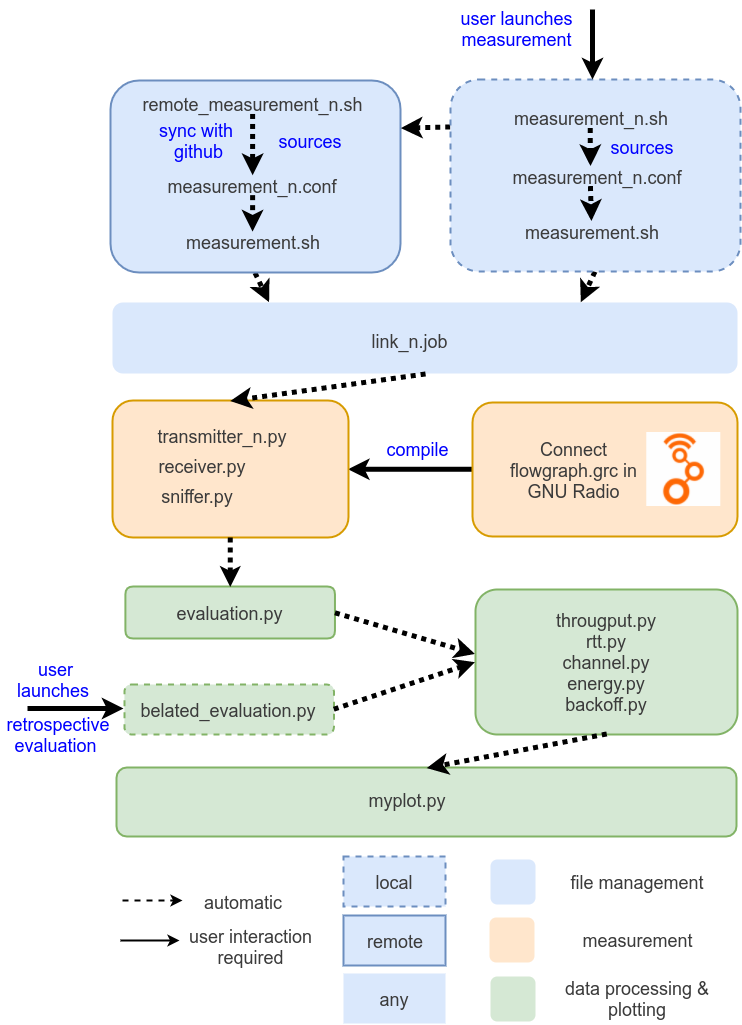
\includegraphics[width=0.5\textwidth]{pictures/script_system}
	\end{center}
	\caption{The three-phase measurement script system.}
\end{figure}

\section{Quality Norms}
\label{sec:quality-standards}

\paragraph{Statistical Reliability}
As mentioned in Section \ref{sec:measurement-scenarios}, each measurement features five repetitions of 100 seconds duration. Compared to a single measurement of 500 seconds this has the downside that script and hardware initialization (about 1.1 seconds per repetition as can be seen in \ref{fig:qa-channel-energy}) has a negative impact on the accuracy of some metrics, particularly throughput, but was easier to implement as this way five data points are provided in a natural way. The statistical quality could be slightly improved by adding more repetitions and increasing the measurement time. 

\paragraph{Data Processing}
Making use of modularity, multiple sets of test data were created for each data processing script (i.e. metric calculation and plotting scripts), provided to and processed by the script and compared with manually calculated results in a similar fashion as GNU Radio quality assurance tests discussed in \cite{gr-python-tut}. Intermediate data processing steps were printed to the console and logged in the log files where applicable. Additionally, experimental results were checked for plausibility. 

\paragraph{Hardware Functionality}
For each device and protocol variation single link baseline measurements were carried out. Not only can we compare the results of device/protocol combinations to two link scenarios, but also assure that the devices are configured and work correctly. RX/TX gains, when necessary, were tweaked each time the hardware was restarted until no or very little ($\le0.2\%$ mean) packet loss was observable in single links scenarios.
Despite all efforts to find a combination of RX/TX gains and distances between nodes, where no packet loss would occur in single link configurations and at the same time the sniffer detects distinct energy levels for each packet type there still remains some degree of imperfection as depicted in Figure \ref{fig:qa-packet-loss}. This problem of packet loss is generally worse for link 1, because it is farther away from the receiver as is shown in Figure \ref{fig:measurement-setup}.  

\begin{figure}[tb]
	\label{fig:qa-packet-loss}
	\begin{center}
		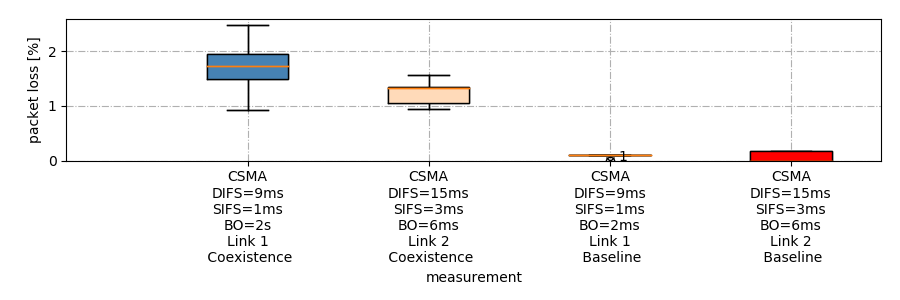
\includegraphics[width=0.9\textwidth]{pictures/qa_packet_loss}
	\end{center}
	\caption[Quality norm packet loss plot.]{Packet loss plot. We only carry out coexistence measurements, if we have less than 0.2\% mean packet loss in the baseline measurements.}
\end{figure}

\begin{figure}[tb]
	\label{fig:qa-channel-energy}
	\begin{center}
		\subfloat[channel energy ]{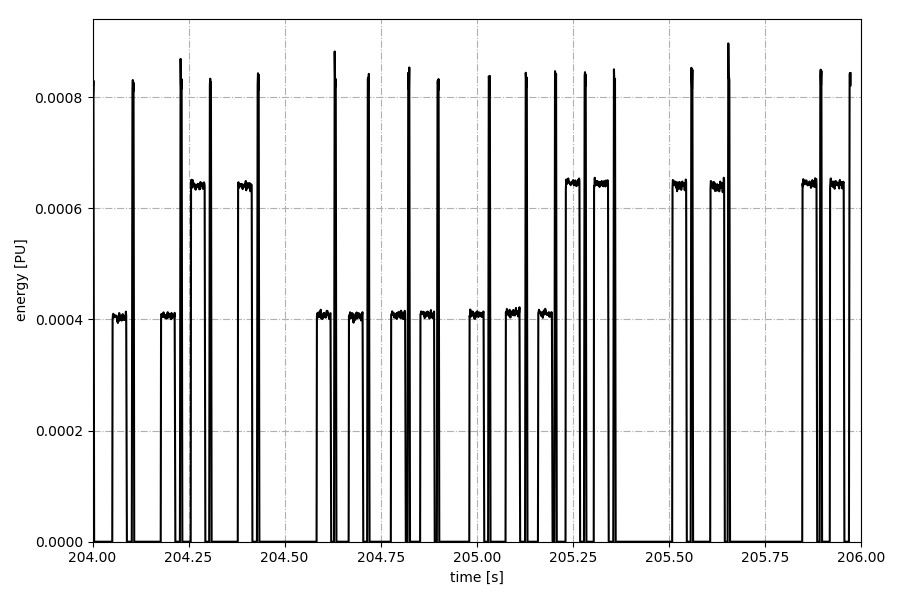
\includegraphics[width=0.9\textwidth]{pictures/qa_channel_energy}}
	\end{center}
	\caption[Quality norm channel energy plot.]{Channel energy plot. The first 1.1 seconds of delay in each measurement repetition are caused by hardware initialization and script delays.}
\end{figure}


\chapter{Measurement Results}
\label{ch:results}

In this chapter we present and discuss the measurement results for different combinations of MAC protocols employed on the two links.  We first assess the measurement results where both senders employ the same MAC protocols. Subsequently, we do the same for several combinations of different MAC protocols. 

\section{Same MAC Protocol For Both Links}
\label{sec:same-protocols}

For the results presented tfhroughout this section, both transmitters executed identical flowgraphs. Generally, when both links use the same MAC protocol we expect to see comparable results for each link over a sufficiently longer period of time, although small variations are also expected due to statistical and hardware-related effects and inaccuracies. 

\subsection{ALOHA}
\label{sec:dbl-aloha}

\begin{figure}[tb]
	\label{fig:results-aloha-dbl-throughput}
	\begin{center}
		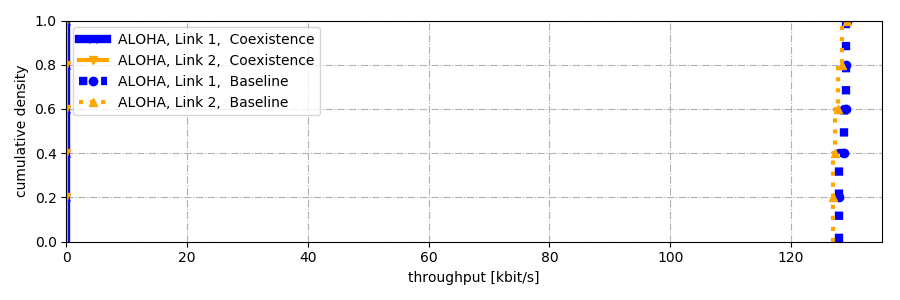
\includegraphics[width=0.9\textwidth]{pictures/results/same_combinations/aloha/throughput_cdf}
	\end{center}
	\caption{Throughput for two links with ALOHA.}
\end{figure}

\begin{figure}[tb]
	\label{fig:results-aloha-dbl-packet-loss}
	\begin{center}
		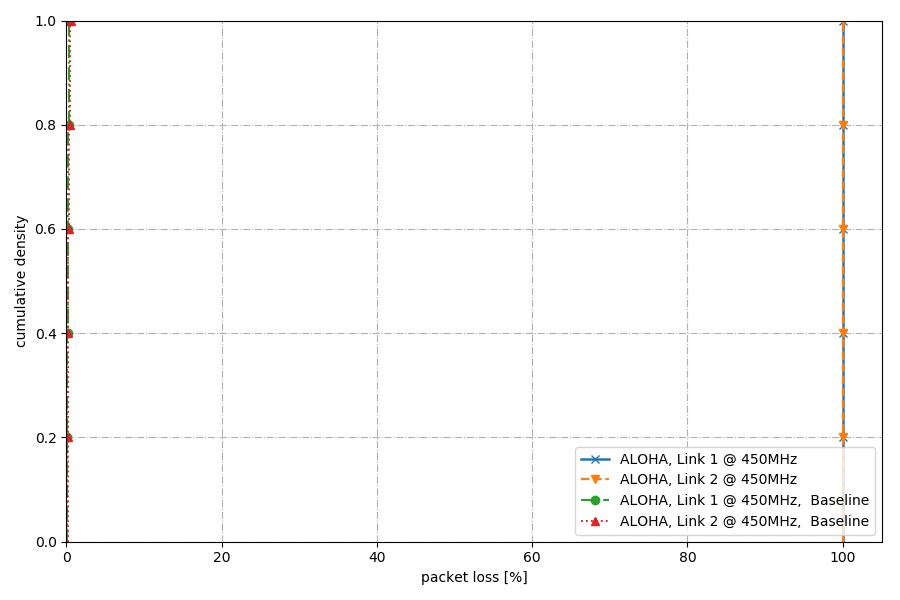
\includegraphics[width=0.9\textwidth]{pictures/results/same_combinations/aloha/packet_loss_cdf}
	\end{center}
	\caption{Packet loss for two links with ALOHA.}
\end{figure}

\begin{figure}[tb]
	\label{fig:results-aloha-dbl-channel-meta}
	\begin{center}
		\subfloat[channel energy CDF]{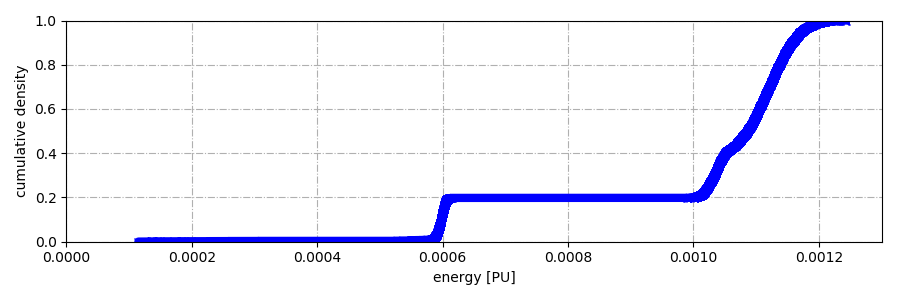
\includegraphics[width=0.9\textwidth]{pictures/results/same_combinations/aloha/smoothed_channel_energy_cdf}\label{fig:results-aloha-dbl-channel-energy-cdf}}
		\\
		\subfloat[channel energy]{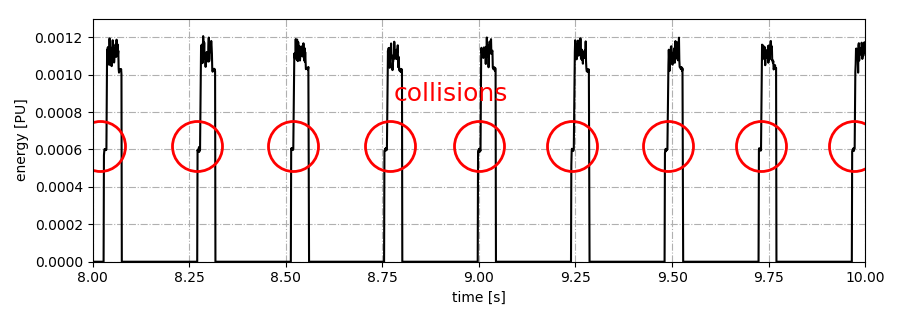
\includegraphics[width=0.9\textwidth]{pictures/results/same_combinations/aloha/smoothed_channel_energy_level_4_line_chart}\label{fig:results-aloha-dbl-channel-energy}}	
	\end{center}
	\caption{Observed channel energy for two links with ALOHA.}
\end{figure}

For two links with saturated ALOHA traffic we expect zero aggregate throughput, since each and every packet collides. Figure \ref{fig:results-aloha-dbl-throughput} confirms this assumption, since both links have zero individual throughput. The corresponding packet loss of 100\% is depicted in Figure \ref{fig:results-aloha-dbl-packet-loss}. A reference value that can be read off Figure \ref{fig:results-aloha-dbl-throughput} is the throughput of a standalone saturated ALOHA link, which is about 130 kbps. This means that the combined throughput of multiple nodes in this channel with the same underlying PHY layer can never exceed 130 kbps and we can assess how well different protocols coexist and how much efficiently they make use of the channel by comparing their aggregated throughput to this value.

Furthermore, a physical view on the channel from the sniffer's perspective is provided in Figure \ref{fig:results-aloha-dbl-channel-meta}\subref{fig:results-aloha-dbl-channel-energy}. Due to the fact that the two transmissions of the senders are not completely overlapping we can see that we do not have a single sender with observed transmission energy level around 0.0011 PU, but instead two transmitters, where the observed energy level of the first transmitter is around 0.0006 PU, which the channel energy CDF in Figure \ref{fig:results-aloha-dbl-channel-meta}\subref{fig:results-aloha-dbl-channel-energy-cdf} confirms. Note that the share of this particular energy (0.0006 PU) in the CDF is so high, because the transmission overlap does not stay constant throughout the whole measurement, but slightly varies with each repetition.

\clearpage

\subsection{CSMA/CA With High Parameter Values}

\begin{figure}[tb]
	\label{fig:results-csma-high-dbl-throughput}
	\begin{center}
		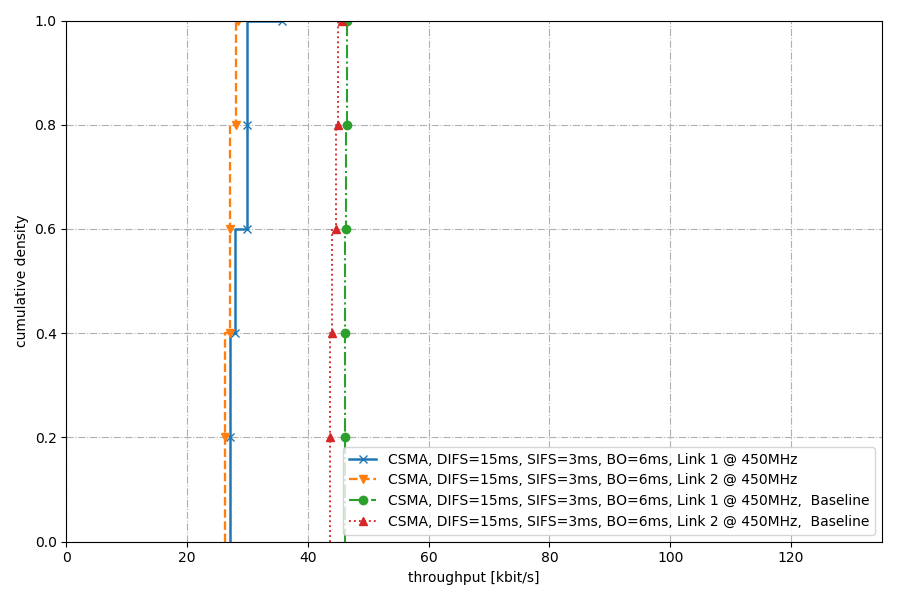
\includegraphics[width=0.9\textwidth]{pictures/results/same_combinations/csma_high_params/throughput_cdf}
	\end{center}
	\caption{Throughput for two links with the high parameter CSMA/CA variant.}
\end{figure}

\begin{figure}[tb]
	\label{fig:results-csma-high-dbl-frame-delay}
	\begin{center}
		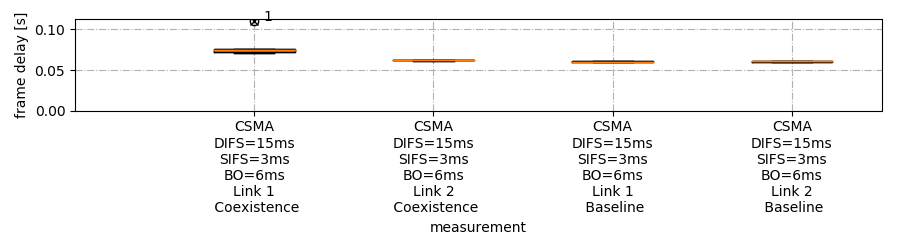
\includegraphics[width=0.9\textwidth]{pictures/results/same_combinations/csma_high_params/frame_delay_boxplot}
	\end{center}
	\caption{Frame delay for two links with the high parameter CSMA/CA variant.}
\end{figure}

\begin{figure}[tb]
	\label{fig:results-csma-high-dbl-backoff}
	\begin{center}
		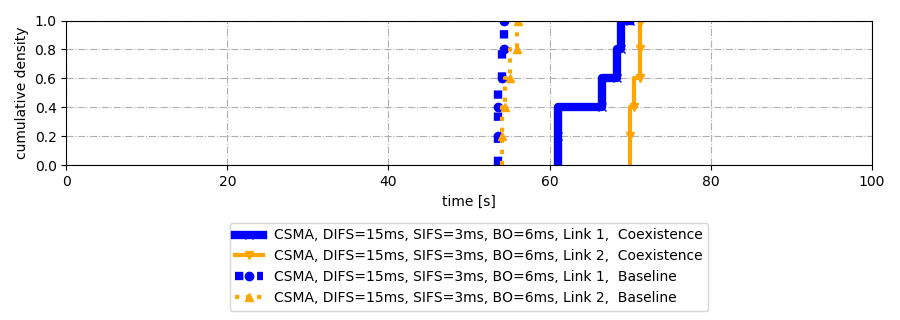
\includegraphics[width=0.9\textwidth]{pictures/results/same_combinations/csma_high_params/backoff_(joint)_sum_cdf}
	\end{center}
	\caption{Backoff for two links with the high parameter CSMA/CA variant.}
\end{figure}

\begin{figure}[tb]
	\label{fig:results-csma-high-dbl-channel-meta}
	\begin{center}
		\subfloat[channel energy CDF]{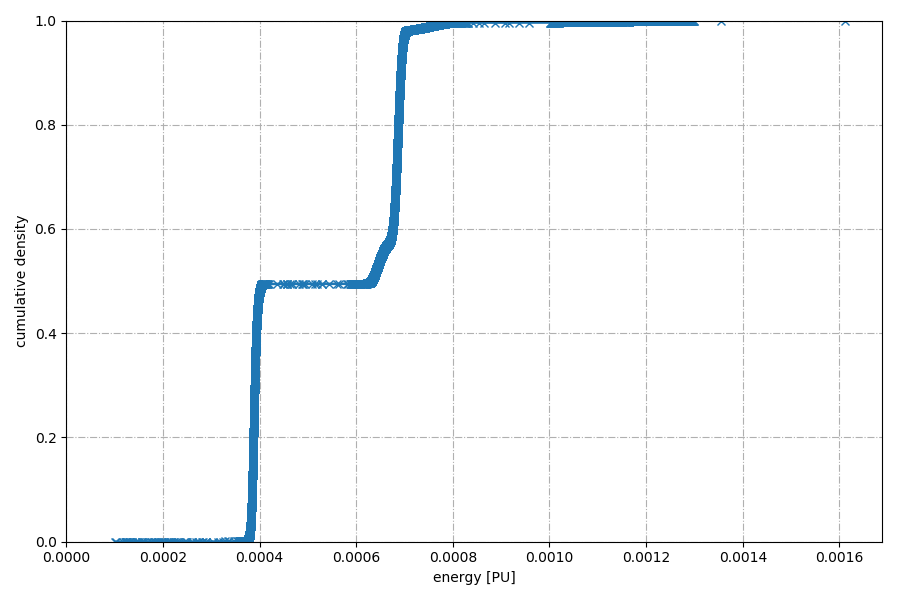
\includegraphics[width=0.9\textwidth]{pictures/results/same_combinations/csma_high_params/smoothed_channel_energy_cdf}\label{fig:results-csma-high-dbl-channel-energy}}
		\\
		\subfloat[channel energy]{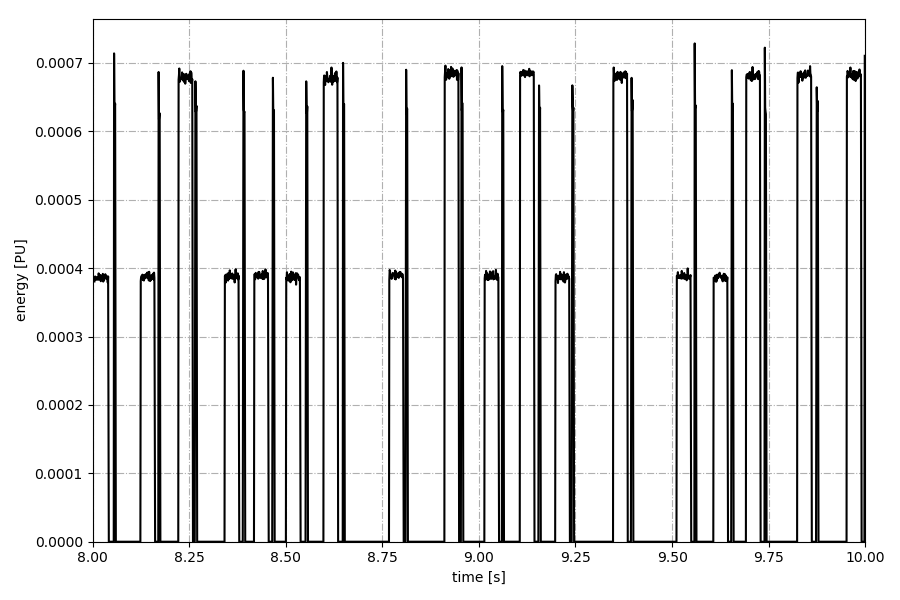
\includegraphics[width=0.9\textwidth]{pictures/results/same_combinations/csma_high_params/smoothed_channel_energy_level_4_line_chart}\label{fig:results-csma-high-dbl-channel-energy-cdf}}
		\\
		\subfloat[logical channel occupation]{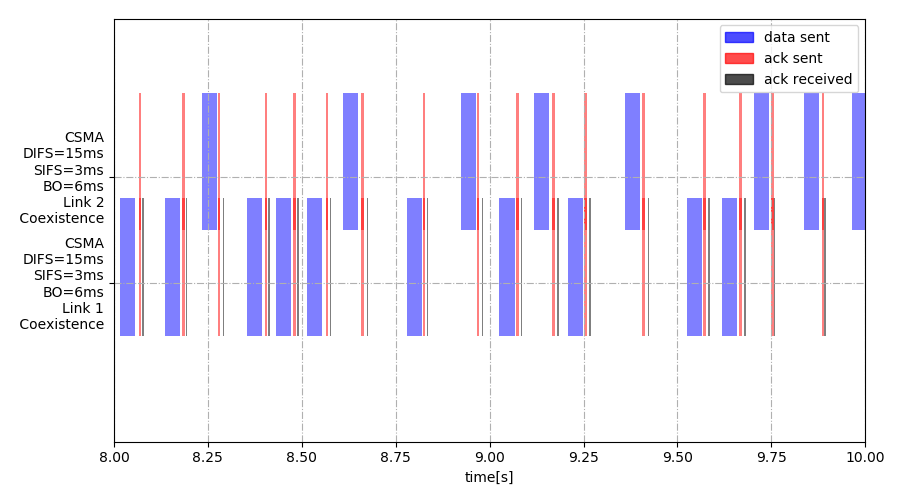
\includegraphics[width=0.9\textwidth]{pictures/results/same_combinations/csma_high_params/zoomed_channel_occupation_gantt_chart}\label{fig:results-csma-high-dbl-channel-occupation}}
	\end{center}
	\caption{Observed channel energy for two links with the high parameter CSMA/CA variant.}
\end{figure}


First of all, with "high parameter values" we mean we chose high values for DIFS, SIFS and backoff slot time (BO), from which we expected that they lead to good coexistence of the two links. In particular, we chose $\text{DIFS}=15 \,\text{ms}$, $\text{SIFS}=3 \,\text{ms}$, $\text{BO}=6 \,\text{ms}$. Figure \ref{fig:results-csma-high-dbl-throughput} shows that the throughput roughly halves (from ) when two links are active at the same time. Figure \ref{fig:results-csma-high-dbl-frame-delay} shows that the frame delay roughly stays the same, where the deviation of the first link comes from packet loss related to hardware problems as described in Section \ref{sec:quality-standards}. Figures \ref{fig:results-csma-high-dbl-channel-meta}\subref{fig:results-csma-low-dbl-channel-energy-cdf}\subref{fig:results-csma-low-dbl-channel-energy} illustrate the same from the sniffer's point of view (POV), as the even throughput among senders is reflected in Figure \subref{fig:results-csma-high-dbl-channel-energy-cdf} with the two observed energy levels of the senders being 0.0004 PU and 0.0007 PU, which is confirmed by Figure \ref{fig:results-csma-high-dbl-channel-energy}. Figure \ref{fig:results-csma-high-dbl-backoff} shows the cumulative backoff times and the logical channel occupation which corresponds to the channel energy plot in Figure \ref{fig:results-csma-high-dbl-channel-meta} \subref{fig:results-csma-high-dbl-channel-energy}. 

\clearpage

\subsection{CSMA/CA With Low Parameter Values}
\label{sec:csma-dbl-low}

\begin{figure}[tb]
	\label{fig:results-csma-low-dbl-throughput}
	\begin{center}
		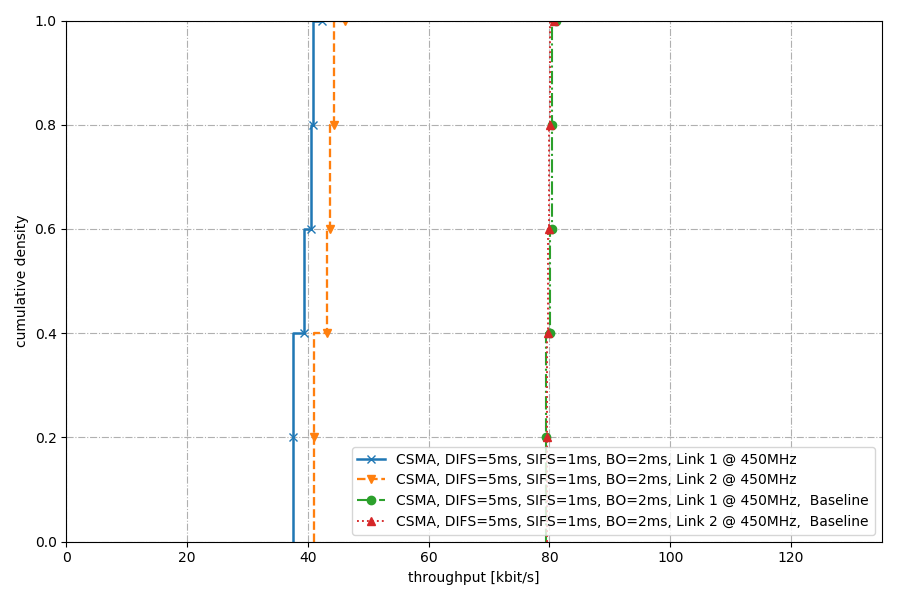
\includegraphics[width=0.9\textwidth]{pictures/results/same_combinations/csma_low_params/throughput_cdf}
	\end{center}
	\caption{Throughput for two links with the low parameter CSMA/CA variant.}
\end{figure}

\begin{figure}[tb]
	\label{fig:results-csma-low-dbl-frame-delay}
	\begin{center}
		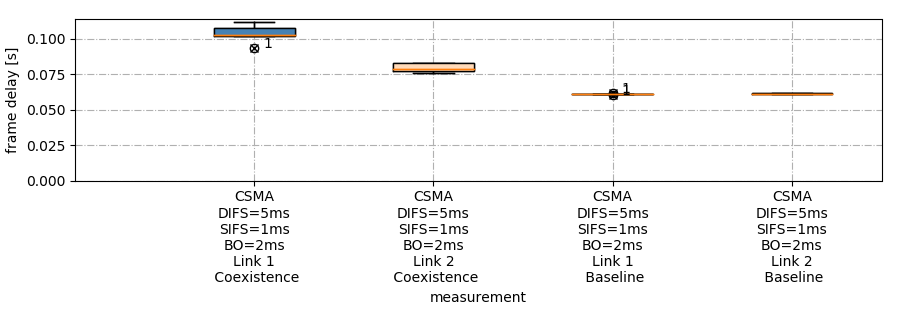
\includegraphics[width=0.9\textwidth]{pictures/results/same_combinations/csma_low_params/frame_delay_boxplot}
	\end{center}
	\caption{Frame delay for two links with the low parameter CSMA/CA variant.}
\end{figure}

\begin{figure}[bt]
	\label{fig:results-csma-low-dbl-backoff}
	\begin{center}
		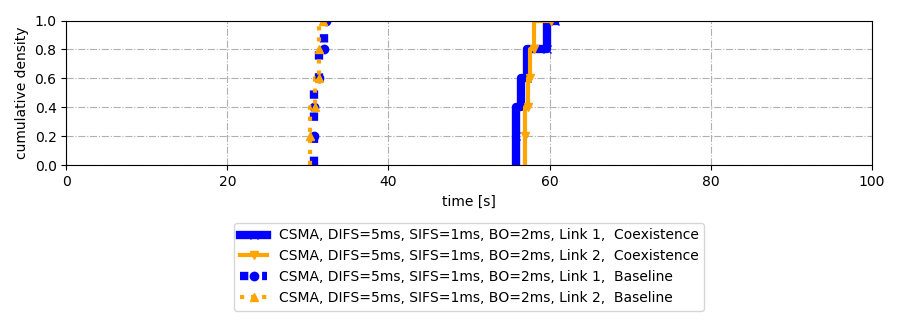
\includegraphics[width=0.9\textwidth]{pictures/results/same_combinations/csma_low_params/backoff_(joint)_sum_cdf}
	\end{center}
	\caption{Backoff times for two links with the low parameter CSMA/CA variant.}
\end{figure}


\begin{figure}[bt]
	\label{fig:results-csma-low-dbl-channel-meta}
	\begin{center}
		\subfloat[channel energy CDF]{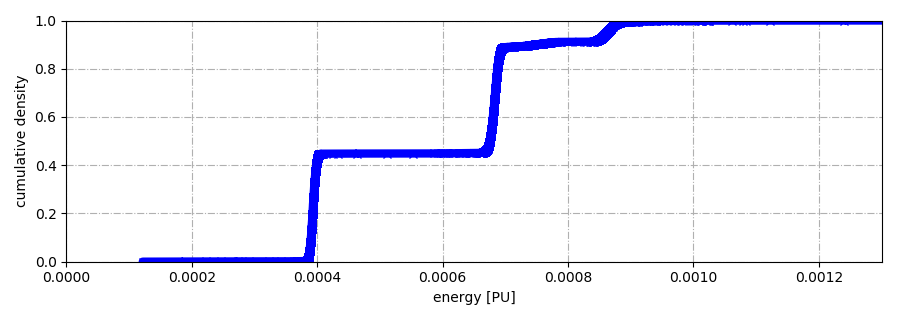
\includegraphics[width=0.9\textwidth]{pictures/results/same_combinations/csma_low_params/smoothed_channel_energy_cdf}\label{fig:results-csma-low-dbl-channel-energy-cdf}}
		\\
		\subfloat[channel energy]{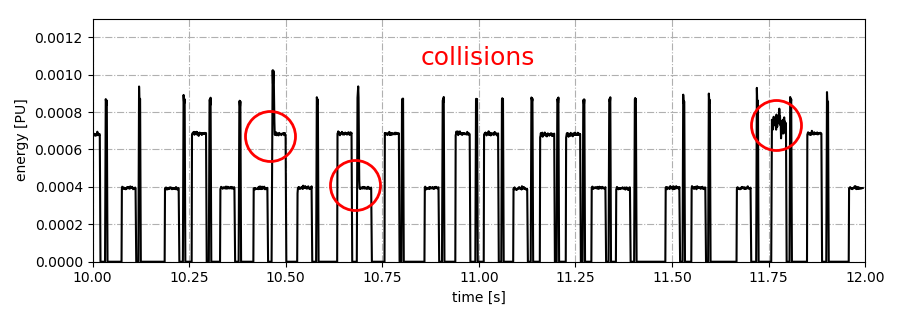
\includegraphics[width=0.9\textwidth]{pictures/results/same_combinations/csma_low_params/smoothed_channel_energy_level_5_line_chart}\label{fig:results-csma-low-dbl-channel-energy}}
		\\
		\subfloat[logical channel occupation]{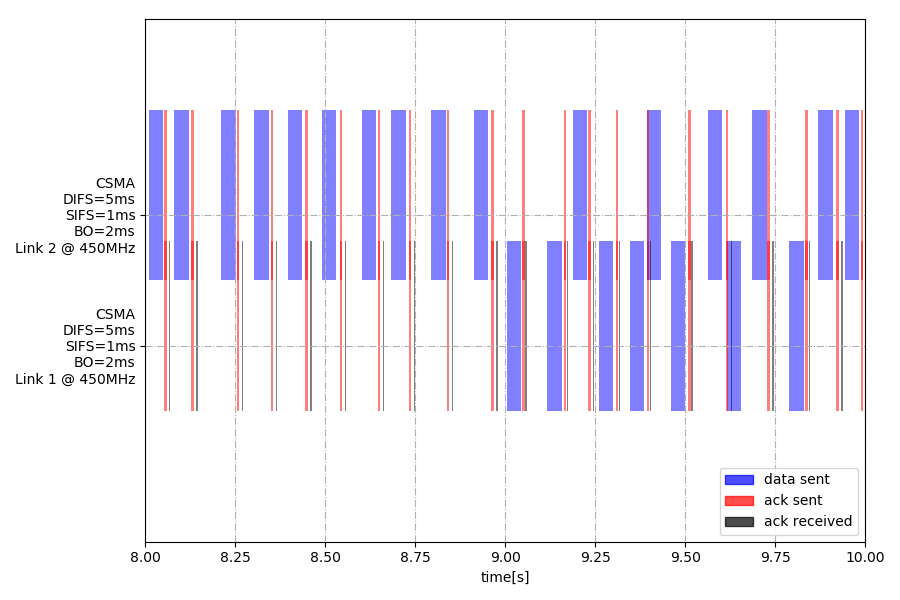
\includegraphics[width=0.9\textwidth]{pictures/results/same_combinations/csma_low_params/zoomed_channel_occupation_gantt_chart}\label{fig:results-csma-low-dbl-channel-occupation}}
	\end{center}
	\caption{Observed channel energy and logical occupation for two links with the low parameter CSMA/CA variant.}
\end{figure}

The next aspect we were interested in is to what extent we can scale down DIFS, SIFS and BO and still retain collision-free transmission. To this end, we reduced the values to $\text{DIFS}=5 \,\text{ms}$, $\text{SIFS}=1 \,\text{ms}$, $\text{BO}=2 \,\text{ms}$\footnote{We chose these values because they are close to the hardware capabilities in terms of time granularity as observed in practice.}. Reducing these values, especially BO increases the throughput, with $CW_\text{min} = 32 \cdot BO$ and uniformly distributed random choice of the backoff slot, we expect a mean delay of $16\cdot BO=32ms$ in the first backoff round, which is rather large compared to DIFS and SIFS.

 Indeed, comparing throughput using the high parameter values (Figure \ref{fig:results-csma-high-dbl-throughput}) with the low parameter values (Figure \ref{fig:results-csma-high-dbl-throughput}) yields a little less than doubled throughput for cutting the backoff. 
 A problem occurs with collisions of ACKs and consecutive data frames of the sender to whom the ACK was not destined caused by the low DIFS in conjunction with hardware delays. Multiple of these collisions occur in the time window depicted in Figure \ref{fig:results-csma-low-dbl-channel-meta}\subref{fig:results-csma-low-dbl-channel-energy}. These collisions lead to the increased frame delays of Figure \ref{fig:results-csma-low-dbl-frame-delay}, where again the additional packet loss of link 1 reflected in the 20ms increased frame delay compared to link 1 is caused by the hardware problems described in Section \ref{sec:quality-standards}.

\clearpage

\subsection{CSMA/CA With Medium Parameter Values}

\begin{figure}[tb]
	\label{fig:results-csma-med-dbl-throughput}
	\begin{center}
		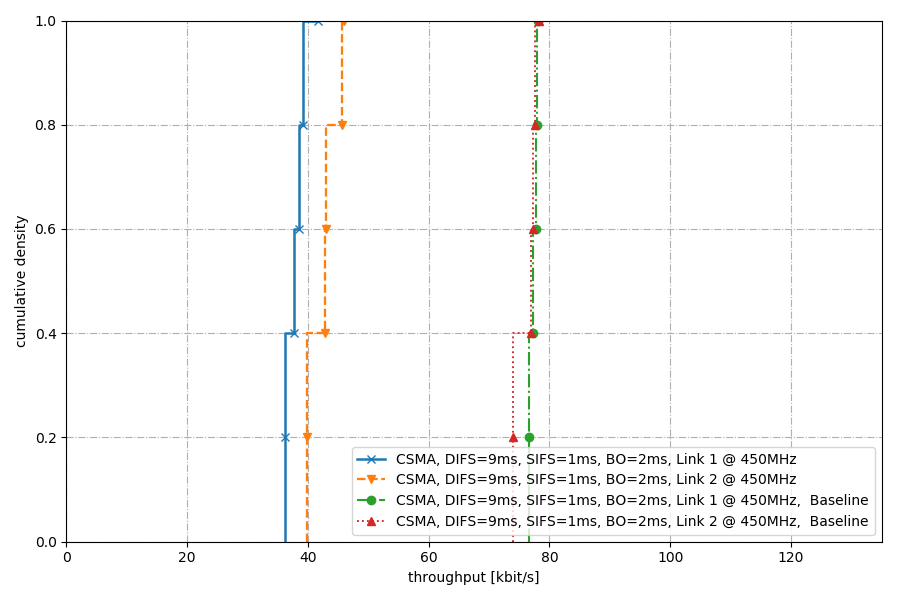
\includegraphics[width=0.9\textwidth]{pictures/results/same_combinations/csma_med_params/throughput_cdf}
	\end{center}
	\caption{Throughput for two links with the medium parameter CSMA/CA variant.}
\end{figure}

\begin{figure}[tb]
	\label{fig:results-csma-med-dbl-frame-delay}
	\begin{center}
		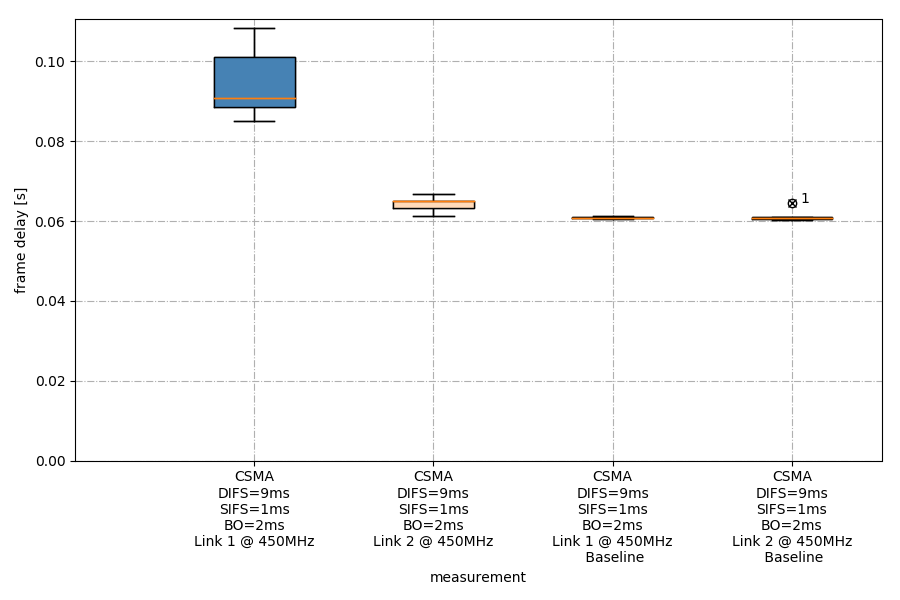
\includegraphics[width=0.9\textwidth]{pictures/results/same_combinations/csma_med_params/frame_delay_boxplot}
	\end{center}
	\caption{Frame delay for two links with the medium parameter CSMA/CA variant.}
\end{figure}

\begin{figure}[tb]
	\label{fig:results-csma-med-dbl-backoff}
	\begin{center}
		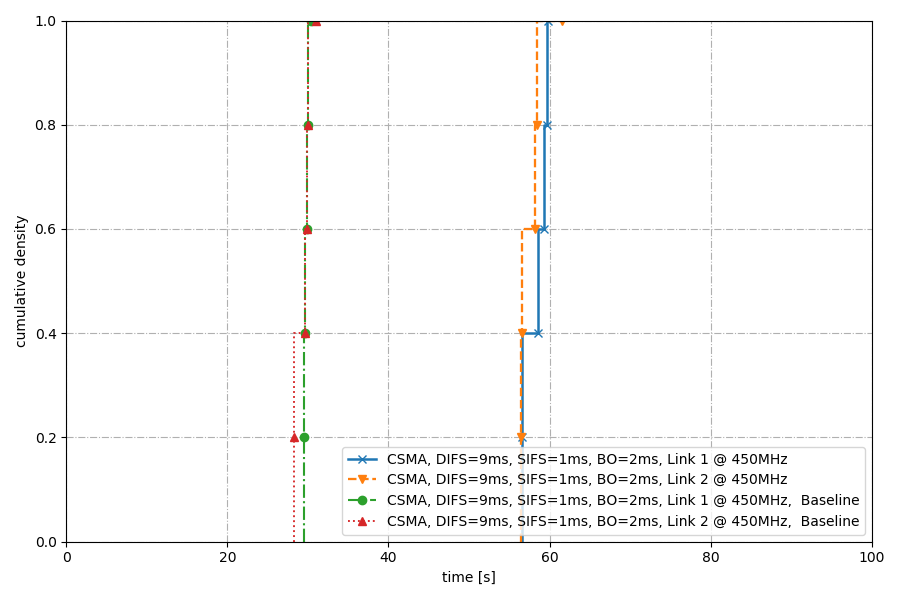
\includegraphics[width=0.9\textwidth]{pictures/results/same_combinations/csma_med_params/backoff_(joint)_sum_cdf}
	\end{center}
	\caption{Backoff times for two links with the medium parameter CSMA/CA variant.}
\end{figure}

\begin{figure}[tb]
	\label{fig:results-csma-med-dbl-channel-meta}
	\begin{center}
		\subfloat[channel energy CDF]{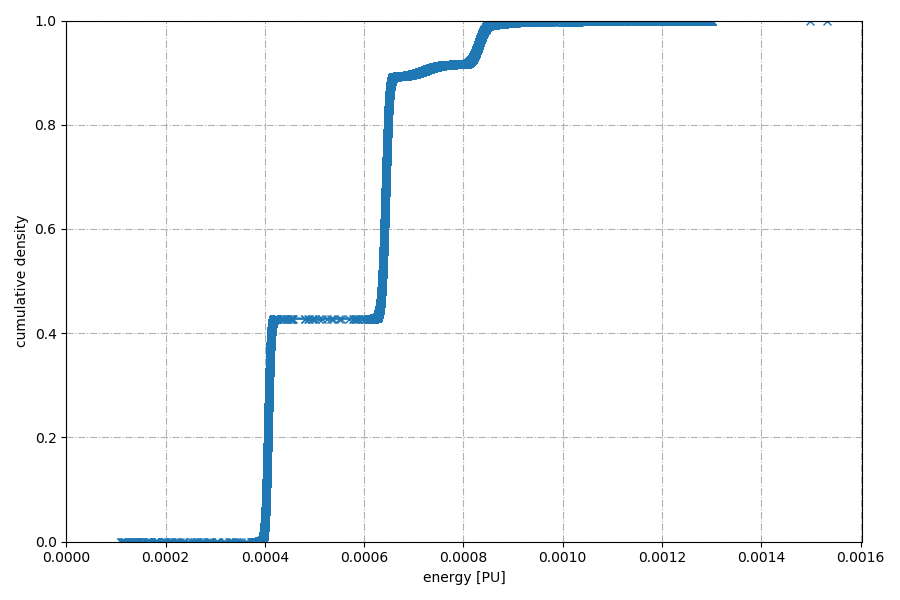
\includegraphics[width=0.84\textwidth]{pictures/results/same_combinations/csma_med_params/smoothed_channel_energy_cdf}}
		\\
		\subfloat[channel energy]{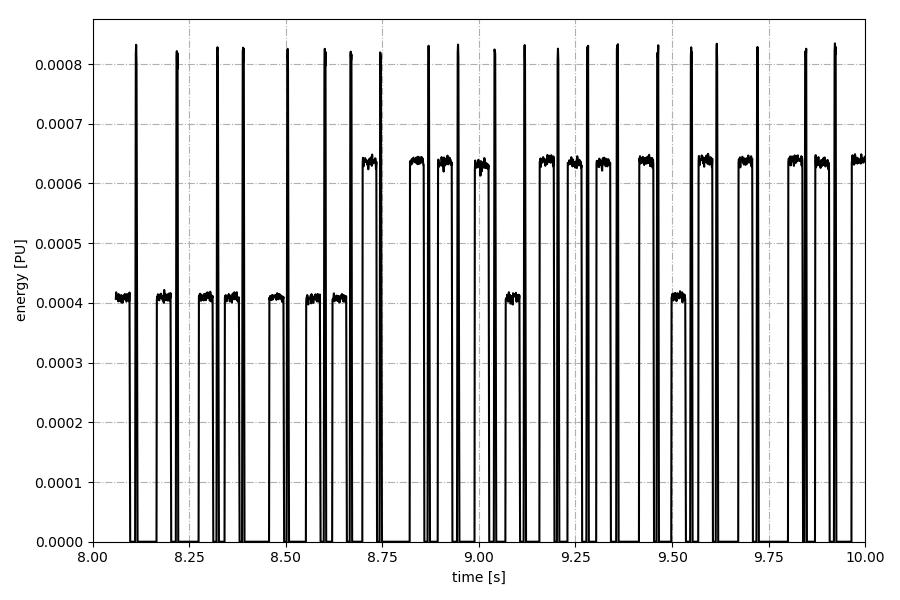
\includegraphics[width=0.84\textwidth]{pictures/results/same_combinations/csma_med_params/smoothed_channel_energy_level_4_line_chart}}
		\\
		\subfloat[logical channel occupation]{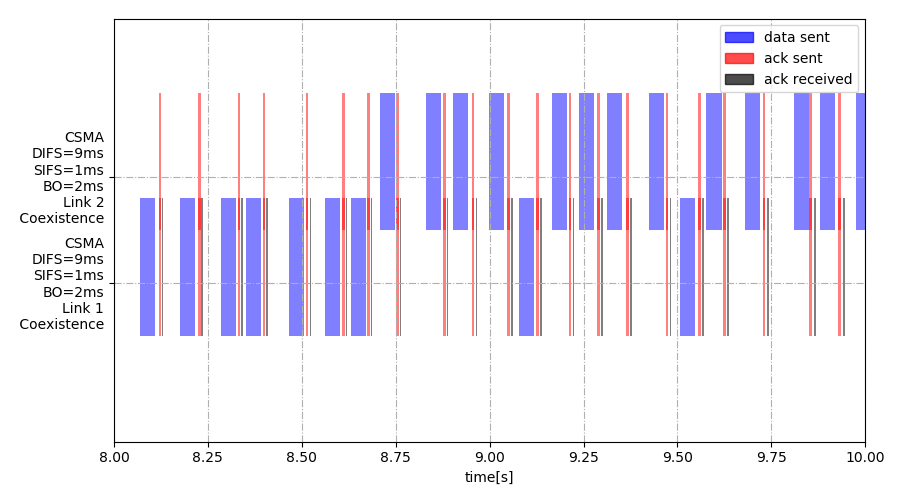
\includegraphics[width=0.84\textwidth]{pictures/results/same_combinations/csma_med_params/zoomed_channel_occupation_gantt_chart}}	
	\end{center}
	\caption{Observed channel energy and logical occupation for two links with the medium parameter CSMA/CA variant.}
\end{figure}

Due to the collisions of ACKs with the data packets of sender 1 as described in Section \ref{sec:csma-dbl-low} we increased DIFS to 9 ms, kept SIFS to 1 ms and BO to 2 ms and indeed, as shown in Figure \ref{fig:results-csma-med-dbl-frame-delay} the frame delay of link 2 is close to the baseline level as result of avoiding collisions. However, since collisions as a result of low DIFS occurred quite infrequently in the last scenario, the metrics (Figures \ref{fig:results-csma-med-dbl-throughput}, \ref{fig:results-csma-med-dbl-backoff}, \ref{fig:results-csma-med-dbl-channel-meta}) roughly stay the same as in the previous scenario (Figures \ref{fig:results-csma-low-dbl-throughput}, \ref{fig:results-csma-low-dbl-backoff}, \ref{fig:results-csma-low-dbl-channel-meta}).

\clearpage

\subsection{1-persistent CSMA}

\begin{figure}[tb]
	\label{fig:results-difs-only-dbl-throughput}
	\begin{center}
		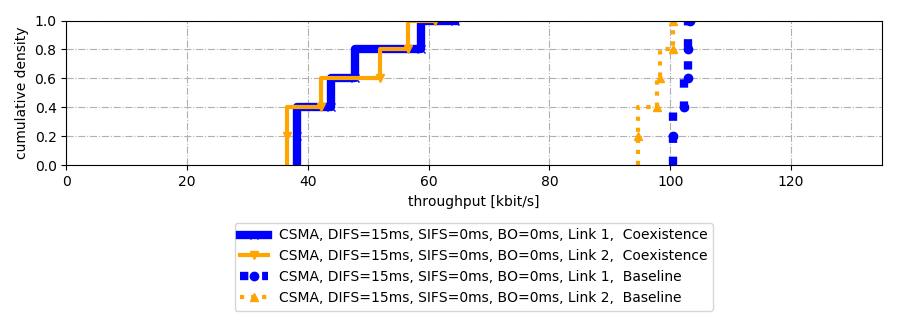
\includegraphics[width=0.9\textwidth]{pictures/results/same_combinations/difs_only/throughput_cdf}
	\end{center}
	\caption{Throughput for two links with 1-persistent CSMA.}
\end{figure}

\begin{figure}[tb]
	\label{fig:results-difs-only-dbl-frame-delay}
	\begin{center}
		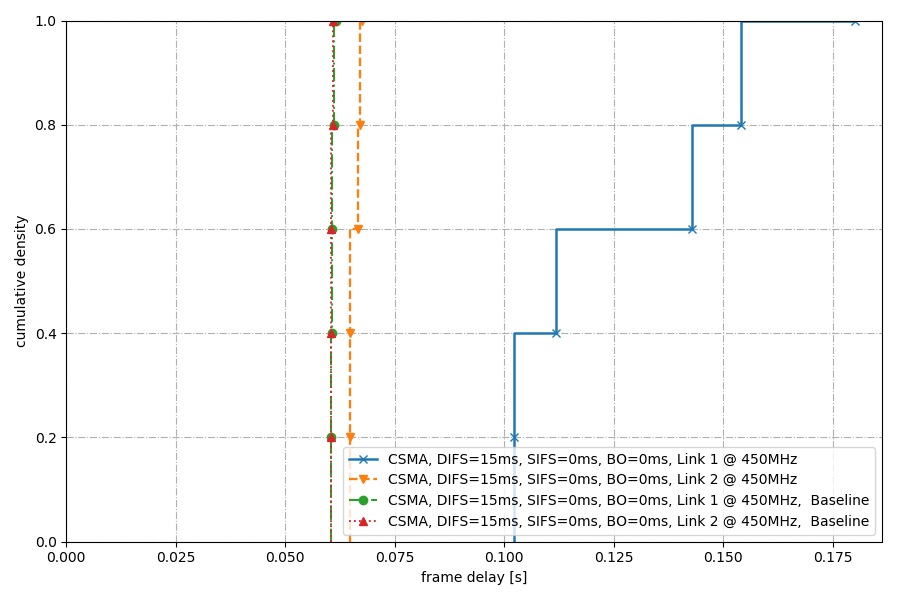
\includegraphics[width=0.9\textwidth]{pictures/results/same_combinations/difs_only/frame_delay_cdf}
	\end{center}
	\caption{Frame delay for two links with 1-persistent CSMA.}
\end{figure}

\begin{figure}[tb]
	\label{fig:results-difs-only-dbl-packet-loss}
	\begin{center}
		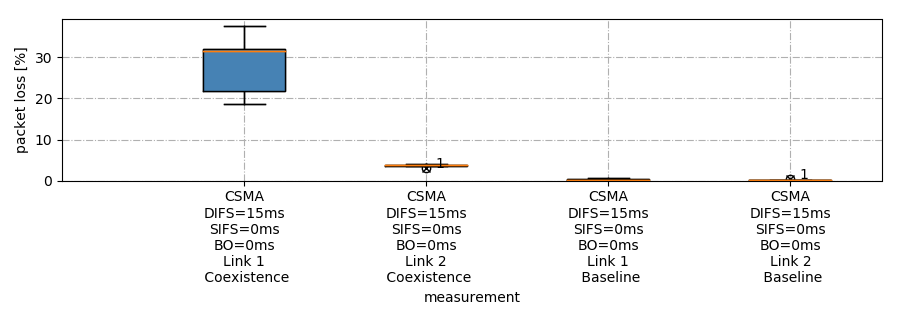
\includegraphics[width=0.9\textwidth]{pictures/results/same_combinations/difs_only/packet_loss_boxplot}
	\end{center}
	\caption{Packet loss for two links with 1-persistent CSMA.}
\end{figure}

\begin{figure}[tb]
	\label{fig:results-difs-only-dbl-channel-meta}
	\begin{center}
		\subfloat[channel energy CDF]{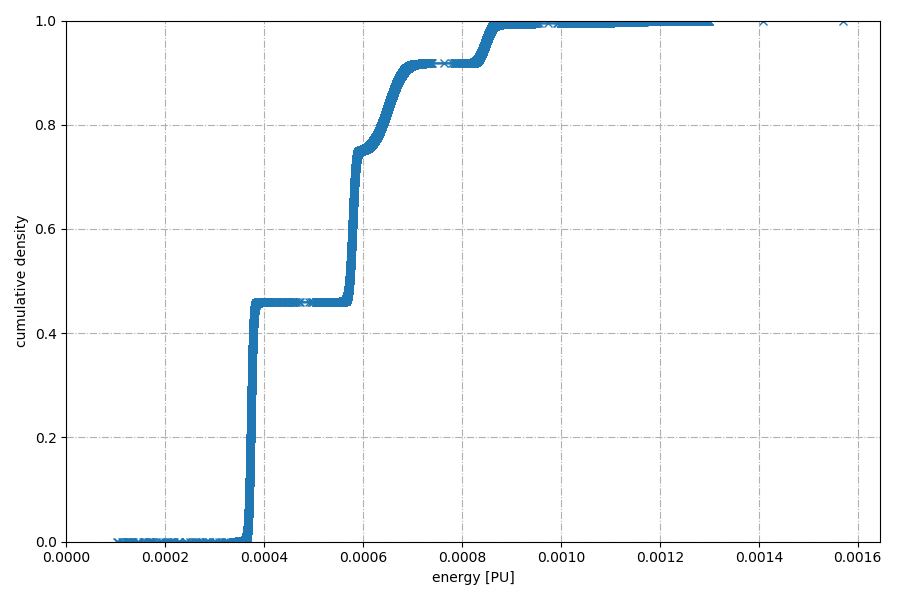
\includegraphics[width=0.9\textwidth]{pictures/results/same_combinations/difs_only/smoothed_channel_energy_cdf}\label{fig:results-difs-only-dbl-channel-energy-cdf}}
		\\
		\subfloat[channel energy]{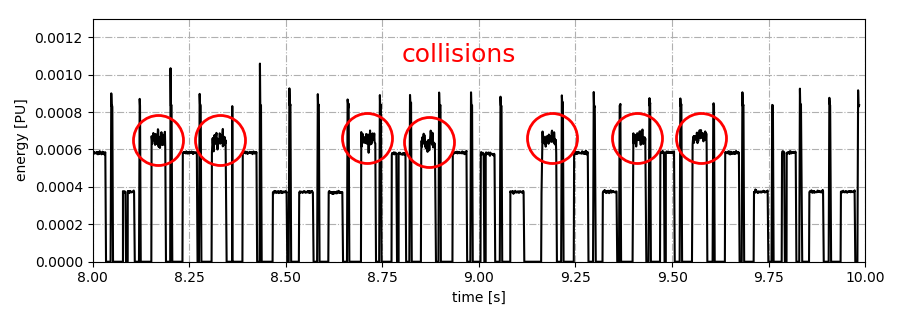
\includegraphics[width=0.9\textwidth]{pictures/results/same_combinations/difs_only/smoothed_channel_energy_level_4_line_chart}\label{fig:results-difs-only-dbl-channel-energy}}
		\\
		\subfloat[logical channel occupation]{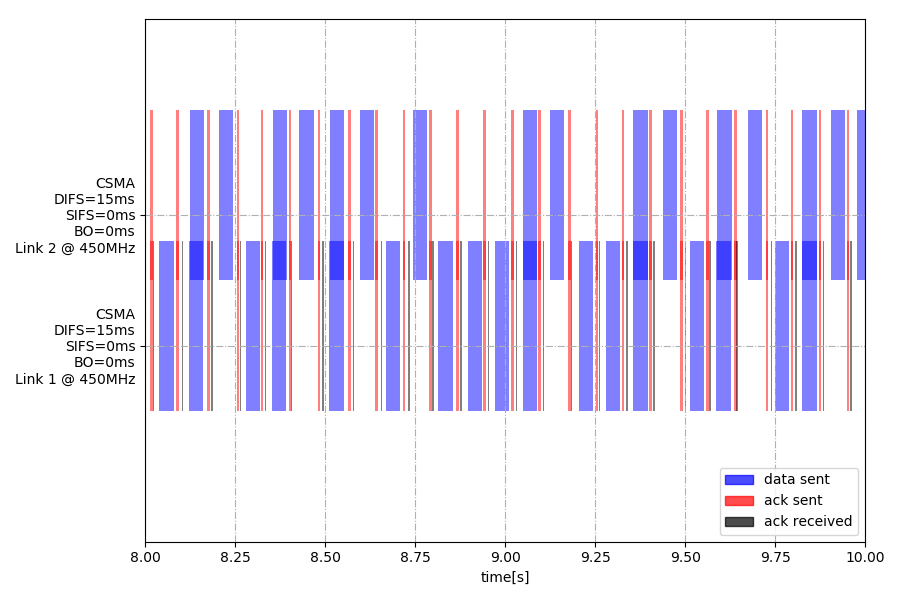
\includegraphics[width=0.9\textwidth]{pictures/results/same_combinations/difs_only/zoomed_channel_occupation_gantt_chart}\label{fig:results-difs-only-dbl-channel-occupation}}
	\end{center}
	\caption{Observed channel energy and logical occupation for two links with 1-persistent CSMA.}
\end{figure}

In the following experiment we examined if a fixed sensing duration of DIFS is enough for harmonious coexistence. As can be seen in Figure \ref{fig:results-difs-only-dbl-channel-meta}\subref{fig:results-difs-only-dbl-channel-occupation} we encounter the problem described in Section \ref{sec:csma-1-persistent}, namely that both\footnote{There are actually three transmitters, since the receiver is transmitting ACKs.} transmitters try to seize the channel at the same time once a sender finished their transmission. If the time granularity of the system was finer, that is to say its timing accuracy was even higher none of the nodes would start to transmit slightly earlier, leading to even further deteriorated throughput than in Figure \ref{fig:results-difs-only-dbl-throughput}. The higher packet loss (Figure \ref{fig:results-difs-only-dbl-packet-loss}) and thus higher frame delay (Figure \ref{fig:results-difs-only-dbl-frame-delay}) of link 1 compared to link 2  can be elucidated by the fact that the signal-to-interference-plus-noise ratio (SINR) ratio of sender 2 is bigger than the SINR of sender 1\footnote{Also, the SINR of the receiver's ACK signal is higher than all others.} as can be surmised from Figure \ref{fig:results-difs-only-dbl-channel-meta}\subref{fig:results-difs-only-dbl-channel-energy}. The extra bend in the channel energy CDF (Figure \ref{fig:results-difs-only-dbl-channel-meta}\subref{fig:results-difs-only-dbl-channel-energy-cdf}) roughly from 0.0006 to 0.0007 PU is a consequence of the interference which is also very visible in Figure \ref{fig:results-difs-only-dbl-channel-meta}\subref{fig:results-difs-only-dbl-channel-energy}.

\clearpage

\section{Different MAC Protocols For Both Links}
\label{sec:different-protocols}

\subsection{ALOHA and CSMA/CA}
\label{sec:aloha-csma}

\begin{figure}[tb]
	\label{fig:results-aloha-csma-throughput}
	\begin{center}
		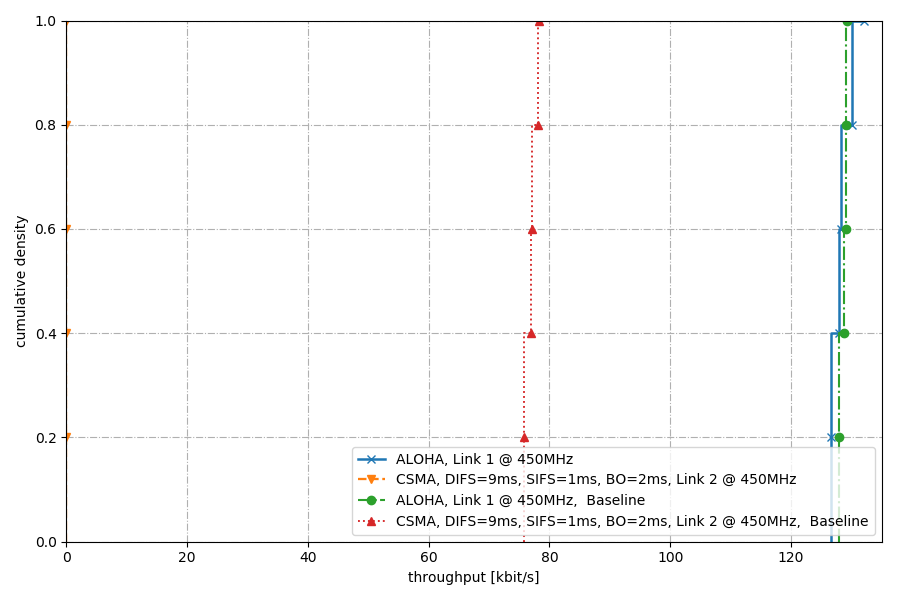
\includegraphics[width=0.9\textwidth]{pictures/results/different_combinations/aloha_csma/throughput_cdf}
	\end{center}
	\caption{Throughput for one link with ALOHA and one link with the medium parameter CSMA/CA variant.}
\end{figure}

\begin{figure}[tb]
	\label{fig:results-aloha-csma-frame-delay}
	\begin{center}
		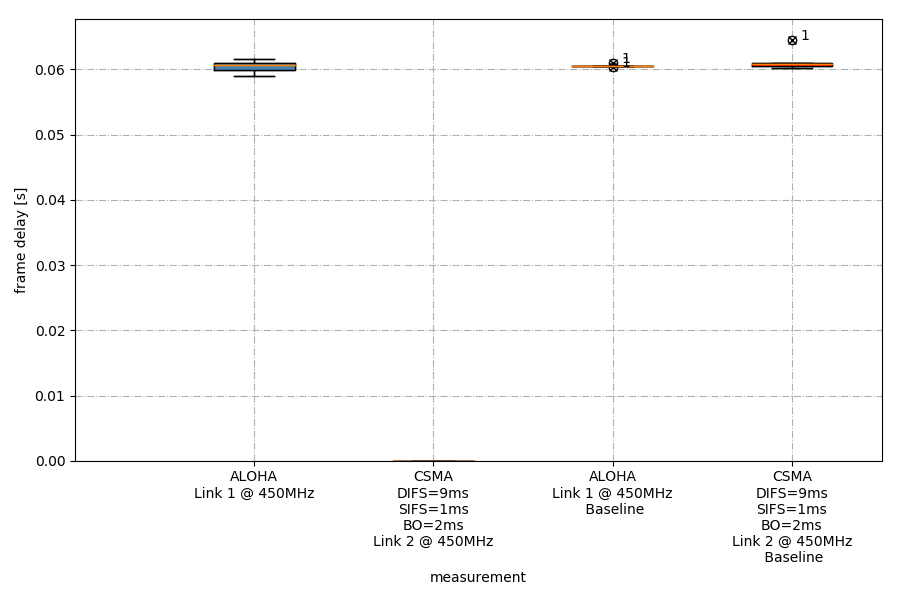
\includegraphics[width=0.9\textwidth]{pictures/results/different_combinations/aloha_csma/frame_delay_boxplot}
	\end{center}
	\caption{Frame delay for one link with ALOHA and one link with the medium parameter CSMA/CA variant.}
\end{figure}

In this experiment we aimed at an experimental confirmation that saturated ALOHA traffic would cause CSMA/CA to stay silent during the whole measurement time. This result is confirmed by Figures \ref{fig:results-aloha-csma-throughput} through \ref{fig:results-aloha-csma-channel-meta}. The throughput and frame delay\footnote{The frame delay is zero, because no frame has ever been sent by the CSMA/CA node.} (Figures \ref{fig:results-aloha-csma-throughput} and \ref{fig:results-aloha-csma-frame-delay}) of CSMA/CA are zero, whereas for saturated ALOHA node throughput and frame delay almost perfectly match the baseline values. The channel energy plots in Figures \ref{fig:results-aloha-csma-channel-meta}\subref{fig:results-aloha-csma-channel-energy} and \ref{fig:results-aloha-csma-channel-meta}\subref{fig:results-aloha-csma-channel-energy-cdf} show that only link 1 and the receiver are transmitting during a time window of 2 s, which also is generally true for the whole measurement duration.

\begin{figure}[bt]
	\label{fig:results-aloha-csma-channel-meta}
	\begin{center}
		\subfloat[channel energy CDF]{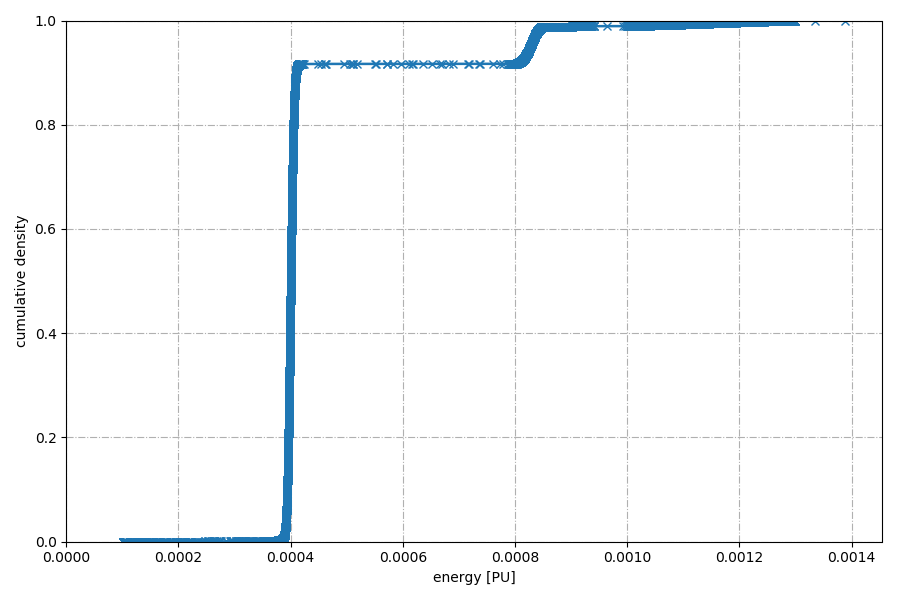
\includegraphics[width=0.9\textwidth]{pictures/results/different_combinations/aloha_csma/smoothed_channel_energy_cdf}\label{fig:results-aloha-csma-channel-energy-cdf}}
		\\
		\subfloat[channel energy]{\includegraphics[width=0.9\textwidth]{pictures/results/different_combinations/aloha_csma/smoothed_channel_energy_level_4_line_chart}\label{fig:results-aloha-csma-channel-energy}}
	\end{center}
	\caption{Observed channel energy for one link with ALOHA and one link with the medium parameter CSMA/CA variant.}
\end{figure}

\clearpage

\subsection{Unsaturated ALOHA and CSMA/CA}
\label{sec:unsat-aloha-csma}

\begin{figure}[tb]
	\label{fig:results-unsat-aloha-csma-throughput}
	\begin{center}
		\includegraphics[width=0.9\textwidth]{pictures/results/different_combinations/aloha_unsat_csma/throughput_cdf}
	\end{center}
	\caption{Throughput for one link with unsaturated ALOHA and one link with the high parameter CSMA/CA variant.}
\end{figure}

\begin{figure}[tb]
	\label{fig:results-unsat-aloha-csma-frame-delay}
	\begin{center}
		\includegraphics[width=0.9\textwidth]{pictures/results/different_combinations/aloha_unsat_csma/frame_delay_cdf}
	\end{center}
	\caption{Frame delay for one link with unsaturated ALOHA and one link with the high parameter CSMA/CA variant.}
\end{figure}

\begin{figure}[tb]
	\label{fig:results-unsat-aloha-csma-packet-loss}
	\begin{center}
		\includegraphics[width=0.9\textwidth]{pictures/results/different_combinations/aloha_unsat_csma/packet_loss_boxplot}	
	\end{center}
	\caption{Packet loss for one link with unsaturated ALOHA and one link with the high parameter CSMA/CA variant.}
\end{figure}

\begin{figure}[tb]
	\label{fig:results-unsat-aloha-csma-channel-meta}
	\begin{center}
		\subfloat[channel energy CDF]{\includegraphics[width=0.9\textwidth]{pictures/results/different_combinations/aloha_unsat_csma/smoothed_channel_energy_cdf}\label{fig:results-unsat-aloha-csma-channel-energy-cdf}}
		\\
		\subfloat[channel energy]{\includegraphics[width=0.9\textwidth]{pictures/results/different_combinations/aloha_unsat_csma/smoothed_channel_energy_level_4_line_chart}\label{fig:results-unsat-aloha-csma-channel-energy}}
		\\
		\subfloat[logical channel occupation]{\includegraphics[width=0.9\textwidth]{pictures/results/different_combinations/aloha_unsat_csma/zoomed_channel_occupation_gantt_chart}\label{fig:results-unsat-aloha-csma-channel-occupation}}
	\end{center}
	\caption{Observed channel energy and logical occupation for one link with unsaturated ALOHA and one link with the high parameter CSMA/CA variant.}
\end{figure}

The next experiment investigates whether relatively low load unsaturated\footnote{We still refer to exponentially distributed time between each packet with $\frac{1}{\lambda}=200ms$, which gives us roughly $G_\text{ALOHA,unsat} \approx \frac{38 \text{kbps}}{130 \text{kbps}}\approx 0.3$, where 38 kbps is the baseline throughput of unsaturated ALOHA and 130 kbps the baseline throughput of saturated ALOHA. We can use this approximation, because the offered channel load of ALOHA is independent from other transmitters and saturated ALOHA approximatively consumes the whole channel capacity.} ALOHA can coexist with CSMA/CA. The throughput of the CSMA/CA sender is reduced to $\frac{18}{45}=40\%$ of the baseline value as depicted in Figure \ref{fig:results-unsat-aloha-csma-throughput}, while the ALOHA throughput approximately remains the same.

Only if the CSMA/CA node transmits a frame before the ALOHA node a collision can occur, which happens during seconds 8-10 of the measurement as shown in Figure \ref{fig:results-unsat-aloha-csma-channel-meta}\subref{fig:results-unsat-aloha-csma-channel-occupation} from a logical POV or in Figure \ref{fig:results-unsat-aloha-csma-channel-meta}\subref{fig:results-unsat-aloha-csma-channel-energy} from a physical POV. With that in mind, we can explain why the frame delay of CSMA/CA varies much more than the frame delay of ALOHA (Figure  \ref{fig:results-unsat-aloha-csma-frame-delay}). The number of ALOHA packets generated during data frame transmission time (or any other period of time) is Poisson-distributed and thus the number of collisions, whereas the likelihood of collision from the POV of an ALOHA frame is dependent on the backoff which in our case is uniformly distributed. The same explanation also applies for the differing variances in packet loss as depicted in Figure \ref{fig:results-unsat-aloha-csma-packet-loss}, whereas the differing values are because ALOHA recklessly pushes its packets into channel, while CSMA/CA does not interfere with ALOHA packets when it senses energy in the channel.

\clearpage

\subsection{Two Variants of CSMA/CA}

\begin{figure}[tb]
	\label{fig:results-csma-15-5-throughput}
	\begin{center}
		\includegraphics[width=0.9\textwidth]{pictures/results/different_combinations/csma_inhomogeneous/15_5/throughput_cdf}
	\end{center}
	\caption{Throughput for one link with the low parameter CSMA/CA variant and one link with the high parameter CSMA/CA variant.}
\end{figure}

\begin{figure}[tb]
	\label{fig:results-csma-15-5-frame-delay}
	\begin{center}
		\includegraphics[width=0.9\textwidth]{pictures/results/different_combinations/csma_inhomogeneous/15_5/frame_delay_boxplot}
	\end{center}
	\caption{Frame delay for one link with the low parameter CSMA/CA variant and one link with the high parameter CSMA/CA variant.}
\end{figure}

\begin{figure}[bt]
	\label{fig:results-csma-15-5-packet-loss}
	\begin{center}
		\includegraphics[width=0.9\textwidth]{pictures/results/different_combinations/csma_inhomogeneous/15_5/packet_loss_boxplot}	
	\end{center}
	\caption{Packet loss for one link with the low parameter CSMA/CA variant and one link with the high parameter CSMA/CA variant.}
\end{figure}

\begin{figure}[bt]
	\label{fig:results-csma-15-5-channel-meta}
	\begin{center}
		\subfloat[channel energy CDF]{\includegraphics[width=0.9\textwidth]{pictures/results/different_combinations/csma_inhomogeneous/15_5/smoothed_channel_energy_cdf}\label{fig:results-csma-15-5-channel-energy-cdf}}
		\\
		\subfloat[channel energy]{\includegraphics[width=0.9\textwidth]{pictures/results/different_combinations/csma_inhomogeneous/15_5/smoothed_channel_energy_level_4_line_chart}\label{fig:results-csma-15-5-channel-energy}}
		\\
		\subfloat[logical channel occupation]{\includegraphics[width=0.9\textwidth]{pictures/results/different_combinations/csma_inhomogeneous/15_5/zoomed_channel_occupation_gantt_chart}\label{fig:results-csma-15-5-channel-occupation}}
	\end{center}
	\caption{Observed channel energy and logical occupation for one link with the low parameter CSMA/CA variant and one link with the high parameter CSMA/CA variant.}
\end{figure}

The goal of our next experiment is to examine how CSMA/CA with different parameter values behave in the same channel. Link 1 uses the low parameter values, whereas link 2 uses the high parameter values. The throughput of link 2 as depicted in Figure \ref{fig:results-csma-15-5-throughput} drops to one seventh of the baseline, whereas it only drops by 20\% for link 1. The reason for this is that with reduced DIFS and BO the chance to grab the channel increases as is shown in Figures \ref{fig:results-csma-15-5-channel-meta}\subref{fig:results-csma-15-5-channel-energy}\subref{fig:results-csma-15-5-channel-energy-cdf}\subref{fig:results-csma-15-5-channel-occupation}. The frame delay increases only marginally as shown in Figure \ref{fig:results-csma-15-5-frame-delay}, which is due to the packet loss depicted in Figure \ref{fig:results-csma-15-5-packet-loss}. The mean packet loss is for link 2 is a little below the expected value of about 1.2\%, whereas for link 1 it is above that value, which is because the SINR of link 2 is higher than for link 1. The expected packet loss comprises of two components. The first component is the baseline packet loss for this measurement, which is around 0.2\%. The second component is the chance that both senders choose the same time to transmit their packet when they sensed the channel idle, which amounts to $ \frac{1}{CW_\text{min}} \cdot \frac{\text{BO}_1}{\text{BO}_2} = \frac{1}{96} \approx 1.0\% $. An idea to reduce the chance of collisions due to this phenomenon is to configure the links to have backoff slot durations that are mutually prime, i.e. have no common divisor, which probably only works if the duration of a backoff slot is big compared to the time granularity of the whole system. 

\clearpage

\subsection{1-persistent CSMA and unsaturated ALOHA}

\begin{figure}[tb]
	\label{fig:results-difs-only-aloha-throughput}
	\begin{center}
		\includegraphics[width=0.9\textwidth]{pictures/results/different_combinations/difs_only_aloha/throughput_cdf}
	\end{center}
	\caption{Throughput for one link with 1-persistent CSMA and one link with unsaturated ALOHA.}
\end{figure}

\begin{figure}[tb]
	\label{fig:results-difs-only-aloha-frame-delay}
	\begin{center}
		\includegraphics[width=0.9\textwidth]{pictures/results/different_combinations/difs_only_aloha/frame_delay_boxplot}	
	\end{center}
	\caption{Frame delay for one link with 1-persistent CSMA and one link with unsaturated ALOHA.}
\end{figure}

\begin{figure}[bt]
	\label{fig:results-difs-only-aloha-packet-loss}
	\begin{center}
		\includegraphics[width=0.9\textwidth]{pictures/results/different_combinations/difs_only_aloha/packet_loss_boxplot}		
	\end{center}
	\caption{Packet loss for one link with 1-persistent CSMA and one link with unsaturated ALOHA.}
\end{figure}

\begin{figure}[bt]
	\label{fig:results-difs-only-aloha-channel-meta}
	\begin{center}
		\subfloat[channel energy CDF]{\includegraphics[width=0.9\textwidth]{pictures/results/different_combinations/difs_only_aloha/smoothed_channel_energy_cdf}\label{fig:results-difs-only-aloha-channel-energy-cdf}}
		\\
		\subfloat[channel energy]{\includegraphics[width=0.9\textwidth]{pictures/results/different_combinations/difs_only_aloha/smoothed_channel_energy_level_4_line_chart}\label{fig:results-difs-only-aloha-channel-energy}}
		\\
		\subfloat[logical channel occupation]{\includegraphics[width=0.9\textwidth]{pictures/results/different_combinations/difs_only_aloha/zoomed_channel_occupation_gantt_chart}\label{fig:results-difs-only-aloha-channel-occupation}}
	\end{center}
	\caption{Observed channel energy and logical occupation for one link with 1-persistent CSMA and one link with unsaturated ALOHA.}
\end{figure}

If there is a link that sends saturated ALOHA traffic through the channel another link will have zero throughput as shown in Sections \ref{sec:dbl-aloha} and \ref{sec:aloha-csma}, which is why we do not consider scenarios with saturated ALOHA traffic anymore. We now discuss a scenario where link 1 uses 1-persistent CSMA and link 2 \emph{unsaturated} ALOHA. In the given scenario it does not make much sense for the CSMA/CA transmitter to back off when the channel is sensed busy either, due to fact that the ALOHA node does not use the LBT mechanism, thus "giving it the chance to transmit" is waste of time as it transmits whenever it wants anyway. Thus, removing the backoff in CSMA/CA promises higher throughput. For this reason we now compare this experiment with the one in Section \ref{sec:unsat-aloha-csma}. The assumption of increased throughput is correct as the comparison between Figures \ref{fig:results-difs-only-aloha-throughput} and \ref{fig:results-aloha-csma-throughput} confirms that removing backoff more than doubles CSMA throughput. It would however, make sense to back off after the reception of an ACK to give the ALOHA node a chance to send a packet. The lack of this backoff explains the increased ALOHA mean packet loss ($\approx 34\%$ total, $\approx 300\%$ increase;  Figure \ref{fig:results-difs-only-aloha-packet-loss}), which is still comparatively low due to the high SINR of the ALOHA node. A representative excerpt of the logical channel occupation is given in Figure \ref{fig:results-difs-only-aloha-channel-meta}\subref{fig:results-difs-only-aloha-channel-occupation}, where only a single ALOHA frame around second 8.8 does not collide with a CSMA packet. The energy plot in Figure  \ref{fig:results-difs-only-aloha-channel-meta}\subref{fig:results-difs-only-aloha-channel-energy} offers a more detailed physical view the channel, where the peak energy level of colliding data packets is not much higher than the energy level of a successful ALOHA transmission. In conjunction with the energy CDF in Figure \ref{fig:results-difs-only-aloha-channel-meta}\subref{fig:results-difs-only-aloha-channel-energy-cdf}, which is taking the whole measurement duration into account and has only a small bend around 0.0006 PU we conclude that if we decrease the TX power of the ALOHA node or use a less robust MCS, such as 64-QAM, ALOHA packet loss would drastically increase. 

\clearpage

\subsection{1-persistent CSMA and CSMA/CA}

\begin{figure}[tb]
	\label{fig:results-difs-only-csma-throughput}
	\begin{center}
		\includegraphics[width=0.9\textwidth]{pictures/results/different_combinations/difs_only_csma/throughput_cdf}
	\end{center}
	\caption{Throughput for one link with 1-persistent CSMA and one link with the high parameter CSMA/CA variant.}
\end{figure}

\begin{figure}[tb]
	\label{fig:results-difs-only-csma-frame-delay}
	\begin{center}
		\includegraphics[width=0.9\textwidth]{pictures/results/different_combinations/difs_only_csma/frame_delay_boxplot}
	\end{center}
	\caption{Frame delay for one link with 1-persistent CSMA and one link with the high parameter CSMA/CA variant.}
\end{figure}

\begin{figure}[tb]
	\label{fig:results-difs-only-csma-channel-meta}
	\begin{center}
		\subfloat[channel energy]{\includegraphics[width=0.9\textwidth]{pictures/results/different_combinations/difs_only_csma/smoothed_channel_energy_level_4_line_chart}\label{fig:results-difs-only-csma-channel-energy}}
		\\
		\subfloat[channel energy CDF]{\includegraphics[width=0.9\textwidth]{pictures/results/different_combinations/difs_only_csma/smoothed_channel_energy_cdf}\label{fig:results-difs-only-csma-channel-energy-cdf}}
	\end{center}
	\caption{Observed channel energy and logical occupation for one link with 1-persistent CSMA and one link with the high parameter CSMA/CA variant.}
\end{figure}

In our last experiment we show that the greedy 1-persistent CSMA approach starves other CSMA/CA links. From the perspective of a CSMA/CA sender it does not matter whether it shares a channel with a saturated 1-persistent CSMA sender or saturated ALOHA sender (Section \ref{sec:aloha-csma}). We can virtually identify no difference in the metrics (Figures \ref{fig:results-difs-only-csma-frame-delay} and \ref{fig:results-difs-only-aloha-channel-meta}\subref{fig:results-difs-only-csma-channel-energy}\subref{fig:results-difs-only-csma-channel-energy-cdf} compared to the corresponding Figures in Section \ref{sec:aloha-csma}) between those combinations except for the reduced throughput \ref{fig:results-difs-only-csma-channel-meta}\subref{fig:results-difs-only-csma-channel-energy-cdf} due to the addition of channel sensing with the duration of DIFS compared to ALOHA. Only if we decreased the offered load of 1-persistent CSMA we could see any and better coexistence\footnote{compared to ALOHA due to the LBT mechanism that stops the 1-persistent CSMA sender from interfering with ongoing transmissions} with CSMA/CA at all.


\chapter{Conclusions and Future Work}
\label{ch:conclusions}

In the final chapter of the thesis, we will summarize the most important conclusions of the preceding Measurement Results chapter and give an outlook on what we think should be subject of future endeavors.

In Section \ref{sec:same-protocols} we showed that two nodes in symmetrical measurement setups, i.e. using the same MAC protocols with the same parameters in a shared channel perform similarly in terms of throughput, frame delay and backoff times where applicable. We showed that two backlogged pure ALOHA nodes recklessly push their packets into the channel resulting in zero throughput. Next, we showed that two CSMA/CA senders with DIFS, SIFS and BO values scaled up from the IEEE 802.11g standard coexist very well with almost collision-free and fair traffic. In an effort to increase throughput, we scaled the values of DIFS, SIFS and BO down and found out that we cannot arbitrarily reduce them without collisions\footnote{other than those resulting from the two nodes by chance transmitting at the same time}, due to the limited system time granularity caused by hardware delays. Solving the resulting optimization problem experimentally yielded $\text{DIFS=9ms}$, $\text{SIFS=1ms}$ and $\text{BO=2ms}$. In the last experiment of said section we proved that renouncing on the backoff mechanism leads to the typical 1-persistent CSMA behavior of multiple senders starting to transmit at the same time, leading to collision and thus high frame delays and high packet loss.

In Section \ref{sec:different-protocols} we examined the coexistence of transmitters employing different MAC protocols. Pro forma we have shown that a single saturated ALOHA sender, rather than two as in Section \ref{sec:same-protocols} is sufficient to lock out other senders from the channel. Consecutively, we showed that even low loads of ALOHA traffic are quite detrimental to the performance of another, in this case a CSMA/CA sender. The next experiment showed that in a scenario with two CSMA/CA senders the backoff slot duration\footnote{provided the minimum backoff window is the same and DIFS is rather small compared to the mean backoff or is scaled with backoff, which is the case in our experiments} is the decisive factor of which fraction of the aggregate throughput each sender gets. Subsequently, we tried to improve on the throughput of CSMA in the unsaturated ALOHA combined with CSMA/CA scenario by replacing the CSMA/CA sender with a 1-persistent CSMA sender, i.e. as a main measure remove the backoff. As a result, the 1-persistent CSMA throughput doubled, whereas the packet loss of ALOHA trippled to about 35\%\footnote{only we should mention, the reason is that SINR of the ALOHA sender was much higher than the SINR of the CSMA/CA sender}. The last experiment shows that from the POV of a CSMA/CA sender it does not make a difference whether it is a saturated 1-persistent CSMA or a saturated ALOHA sender occupying the shared channel.    

Eventually, we want to give an outlook on future work proceeding from questions undiscussed in this thesis. Going from our last experiment as a starting point it would interesting to see how much better 1-persistent CSMA fares compared to ALOHA in lower load situations concerning coexistence with CSMA/CA. More important and probably more practical questions are how the backoff mechanism can be enhanced to adaptively accommodate different traffic situations without introducing uneconomical complexity. One idea is to modify the CW growth by taking the CW of previous transmissions into account or to use a different growth scheme, e.g. linear instead of binary exponential. Other ideas are using different and/or adaptive backoff slot durations for different nodes in the network or changing minimum contention windows all in order to further reduce the chance that multiple nodes start sending at \emph{exact} same time, while simultaneously keeping unnecessary waiting times at bay. A completely different approach is to study the effect of transmission power, which may adaptively be varied to limit the range of a sender in order to allow a greater number of transmissions in the environment. On the other hand TX power could be adaptively increased if a node has priority traffic, allowing collisions to send traffic through a channel that is otherwise saturated. 


\appendix
\chapter{Bash and Python Scripts}

This appendix aims at giving in-depth insight in the scripts used in the three phases of the measuring, data processing and plotting process. The basic principle, however, is depicted in section \ref{sec:script-system}. Minor edits were made for format and aesthetic reasons.

\begin{lstlisting}[language=Bash,caption=measure.sh]
echo "remote_measurement is set to "$remote_measurement"."

function setup_remote_connection
{
  reset
  sshpass -p "inets" ssh -$remote_flags $remote_user@$remote_ip "bash -s" < remote_measurement_$link.sh
}

function prepare_measurement
{
    reset
    measurement_counter=0
    ## let's make sure all the directories exist
    printf "\nchecking if paths exists...\n"

    #let's first make absolutely sure the raw data source path exists
    if [ ! -d $raw_data_source_path ];
      then
        mkdir -p $raw_data_source_path
        echo $raw_data_source_path" created."
      else
        rm -r $raw_data_source_path/*
    fi

    if [ -d $plot_directory_path ];
      then
        echo $plot_directory_path" already existed!"
        cd $plot_directory_path
        # create measurement directory
        while [ -d $measurement_counter ]; do
            measurement_counter=$(($measurement_counter+1))
        done
        export measurement_counter;
    fi

    if [ -d $log_path ];
      then
        echo $log_path" already existed!"
      else
        mkdir -p $log_path
        echo $log_path" directory created."
    fi

    mkdir -p $plot_directory_path/$measurement_counter
    echo $plot_directory_path/$measurement_counter" directory created."

    mkdir -p $data_source_path/$measurement_counter
    echo $data_source_path/$measurement_counter" directory created."

    mkdir -p $jobs_open_path
    mkdir -p $jobs_done_path

    ## let's check if measurement script is defined
    # if $measurement_scripts undefined:
    # go through directory and list all python files
    if [ -z ${measurement_scripts+x} ];
      then
        echo  "no measurement scripts set,
              going through files inside of $locate_base_path."
        echo "please add a the full path of one of the files to \$scritps."
        #locate -r "$locate_base_path" | grep "\.py$"
        echo "terminated. ding dong"
        exit -1
    fi

    printf "\n"
}

function measure
{
  local prematurely_aborted=0

  for ((x = 1 ; x <= $measurement_repetitions ; x += 1)); do

    # get pid to later kill it
    for i in "${measurement_scripts[@]}"
    do
      python $measurement_script_path/$i &
      #measurement_scripts_pid+=($!)
    done

    for ((y = $timer ; y > 0 ; y -= 1)); do
      echo "measurement $x/$measurement_repetitions complete in $y second(s)."
      if [ $check_if_prematurely_aborted -eq 1 ];
        then
          if $(ps -p ${measurement_scripts_pid[*]}) | grep ${measurement_scripts_pid[*]};
            then
              :
            else
              prematurely_aborted=1
              echo  "Scripts were killed prematurely. Measurement may be incomplete."
              break
          fi
      fi
      sleep 1
    done

    kill $(jobs -p)

    # save this measurement's data to special folder
    mkdir -p $data_source_path/$measurement_counter/$x
    echo  "measurement $x raw data directory created $data_source_path/$measurement_counter/$x/."

    echo $raw_data_source_path
    echo $(ls $raw_data_source_path | egrep "*_$link.txt")

    cd $raw_data_source_path
    mv -v $(ls | egrep "*_$link.txt") $data_source_path/$measurement_counter/$x/
    cp -v $(ls | egrep "sniffer") $data_source_path/$measurement_counter/$x/
    if [ "$receiver_mode" == "single" ];
      then
        cp -v $(ls | egrep "receiver") $data_source_path/$measurement_counter/$x/
    fi
    echo  "measurement $x raw data moved to $data_source_path/$measurement_counter/$x/."
    printf "\n"
    # will only ever be true if $check_if_prematurely_aborted is set to 1
    if [ $prematurely_aborted -eq 1 ];
      then
        if [ $plot_if_prematurely_aborted -eq 0 ];
          then
            echo "plotting if measurement prematurely aborted set to false."
            echo "terminated."
            exit -1
        fi
    fi

  done

  #exit remote connection
  if [ $remote_measurement -eq 1 ]; then
    echo "remote_measurement is set to "$remote_measurement"."
    exit
  fi
}

function plot
{
  ## plot the results
  echo "now processing results..."

  # call the plotting scripts as data
  #echo "starting to generate plots..."
  echo "plotting python should be: "$plot_py" ("$os")."

  for i in ${plot_scripts[@]}; do
    bash -c "$plot_py $plot_py_path/$i"
  done

  printf "\n"
  echo "+--------------------+"
  echo "| plotting completed |"
  echo "+--------------------+"
}

function cleanup
{
    ##cleaning up the mess you created!
    #kill all child proceesses
    echo "staring cleanup..."
    echo "killing all lingering child processes..."
    killall -9 -g $0
    cd $this_path
    exit
}
trap cleanup sighup sigint sigkill;
trap "cd $this_path" exit;

function main
{
  # clear up console
  #reset
  # check if jobs_open directory is empty
  if [ ! "$(ls -a $jobs_open_path)" ]; then
    echo "there seem to be no open jobs. measuring with default parameters."
    prepare_measurement
    #take measurements
    measure | tee -a $log_path/default_$measurement_counter.log
    # create plot if desired
    if [ $plot_enabled -eq 1 ]; then
      plot | tee -a $log_path/default_$measurement_counter.log; fi
  else
    prepare_measurement
    echo "open jobs detected! let's get to work..."
    jobs=$jobs_open_path/*
    for job in $jobs; do
      source $job;
      job_name=$(echo $job | rev | cut -d"/" -f1 | rev )
      log=$log_path/$job_name"_"$measurement_counter.log
      #echo $job_name
      cat $job | tee -a $log
      cat measurement_$link.conf | tee -a $log
      measure | tee -a $log
      if [ $plot_enabled -eq 1 ]; then
        plot | tee -a $log
      fi
      if [ $move_after_job_done -eq 1 ]; then
        cp $job $plot_directory_path/$measurement_counter/
        mv $job $jobs_done_path/
      fi
      export measurement_counter=$((measurement_counter++))
    done
  fi
}

if [ $debug_mode -eq 1 ]; then
  printf "\n"
  echo "+----------------------+"
  echo "| debug mode is active.|"
  echo "+----------------------+"
fi

if [ $remote_measurement -eq 1 ]; then
  # call to main included here
    setup_remote_connection
  else
    main
fi

\end{lstlisting}

\begin{lstlisting}[language=Python,caption=evaluation.py]
import numpy as np
import myplot
import os

import rtt
import throughput as tp
import channel_occupation
import backoff
import sniffer

# From Bash
measurement = [int(os.environ["measurement_counter"])]
links = [int(os.environ["link"])]
repetitions = int(os.environ["measurement_repetitions"])
data_source_path = os.environ["data_source_path"]
plot_path = os.environ["plot_directory_path"]+"/"+os.environ["measurement_counter"]+"/"
plot_type = ["cdf", "boxplot"]
throughput_data_files = os.environ["throughput_data_files"].split(",")
rtt_data_files = os.environ["rtt_data_files"].split(",")
co_data_files = os.environ["co_data_files"].split(",")
sniffer_data_files = os.environ["sniffer_data_files"].split(",")
retxs_data_files = os.environ["retxs_data_files"].split(",")
show_plot = int(os.environ["show_plot_after_measurement"])
rtt_mode = os.environ["rtt_mode"]
max_retxs = 6
eval_mode = "live"
timer = int(os.environ["timer"])
receiver_mode = os.environ["receiver_mode"]

#From Python
plot_pdf = False
boxplot_xticks = [ "measurement "+str(index) for index in measurement ]
legend_labels = [ tick.replace("\n", ", ") for tick in boxplot_xticks ]

custom_legend_coordinates = {
    "rtt":                 [0.24,0.85,"upper left"],
    "packet_loss":         [1,0,"lower right"],
    "retxs":               [1,0,"lower right"],
    "throughput":          [1,0,"lower right"],
    "diagnosis_sender":    [1,0,"lower right"],
    "diagnosis_receiver":  [1,0,"lower right"],
    "backoff":             [1,0,"lower right"],
    "channel_occupation":  [1,0,"lower right"],
    "sniffer":             [1,0,"lower right"]
}

create_plots = {
    "rtt":                  False,
    "packet_loss":          False,
    "retxs":                False,
    "throughput":           True,
    "diagnostic":           True,
    "backoff":              True,
    "channel_occupation":   True,
    "sniffer":              True
}

channel_occupation_mode = {
    "occupation_mode":  ["overview", "zoom"],
    "zoom":             [5,7],
    "zoom_mode":        "interval",
    "zoom_interval":    2
}

sniffer_settings =  {
    "sniffer_mode":             ["physical", "smoothed"],
    "link":                     1,
    "zoom":                     [0.0,timer*repetitions],
    "zoom_mode":                "interval",
    "zoom_interval":            2,
    "smoothing_difference":     0.0001,
    "smoothing_derivative":     0.01,
    "smoothing_range":          [0.0010,0.0013]
}

#Unimplemented, use later
annotations_below   = []
annotations_other   = []

eval_dict = {
    "measurement":              measurement,
    "repetitions":              repetitions,
    "data_source_path":         data_source_path,
    "xticks":                   boxplot_xticks,
    "legend":                   legend_labels,
    "annotations_below":        annotations_below,
    "annotations_other":        annotations_other,
    "throughput_data_files":    throughput_data_files,
    "retxs_data_files":         retxs_data_files,
    "rtt_data_files":           rtt_data_files,
    "show_plot":                show_plot,
    "legend_coordinates":       custom_legend_coordinates,
    "create_plots":             create_plots,
    "links":                    links,
    "rtt_mode":                 rtt_mode,
    "channel_occupation_mode":  channel_occupation_mode,
    "co_data_files":            co_data_files,
    "sniffer_data_files":       sniffer_data_files,
    "sniffer_settings":         sniffer_settings,
    "timer":                    timer,
    "plot_pdf":                 plot_pdf
}

for index,a_plot_type in enumerate(plot_type):
    if plot_type[index] == "cdf":
        grid                = True
    else:
        grid                = True

    eval_dict["plot_type"]  = [plot_type[index]]
    eval_dict["plot_path"]  = plot_path
    eval_dict["grid"]       = grid

    if create_plots["backoff"] == True:
        print("Creating backoff plot!")
        backoff.backoff(**eval_dict).plot()
    if create_plots["rtt"] == True:
        print("Creating rtt plot!")
        rtt.rtt(**eval_dict).plot()
    if create_plots["throughput"] == True:
        print("Creating throughput plot!")
        tp.tp(**eval_dict).plot()

# The plots with only one plot type!
if create_plots["channel_occupation"] == True:
    print("Creating channel occupation plot!")
    channel_occupation.channel_occupation(**eval_dict)
if create_plots["sniffer"] == True:
    print("Creating sniffer energy plot!")
    sniffer.sniffer(**eval_dict)

print("Done.")
\end{lstlisting}
\chapter{Abbreviations}

\begin{acronym}
\acro{AM}{amplitude modulation}
\acro{BMAC}{Berkeley MAC}
\acro{CCA}{clear channel assessment}
\acro{CDMA}{code division multiple access}
\acro{CSMA}{carrier sense multiple access}
\acro{CSMA/CA}{CSMA with collision avoidance}
\acro{CSMA/CD}{CSMA with collision detection}
\acro{CTS}{clear to send}
\acro{DCF}{distributed coordination function}
\acro{DIFS}{DCF interframe spacing}
\acro{DIY}{do it yourself}
\acro{EIFS}{extended interframe spacing}
\acro{FDMA}{Frequency Division Multiple Access}
\acro{FM}{frequency modulation}
\acro{GNU}{GNU is not Unix}
\acro{GR}{GNU Radio}
\acro{GRC}{GNU Radio Companion}
\acro{GUI}{graphical user interface}
\acro{LabVIEW}{Laboratory Virtual Instrumentation Engineering Workbench}
\acro{LAN}{local area network}
\acro{LLC}{logical link control}
\acro{LBT}{listen before talk}
\acro{MAC}{medium access control}
\acro{NAV}{network allocation vector}
\acro{PCF}{point coordination function}
\acro{PDU}{packet data unit}
\acro{PHY}{physical (layer)}
\acro{PIFS}{PCF interframe spacing}
\acro{PMT}{polymorphic type}
\acro{QPSK}{quadrature phase-shift keying}
\acro{RF}{radio frequency}
\acro{RTS}{request to send}
\acro{SDK}{software development kit}
\acro{SMAC}{Sensor MAC}
\acro{SDR}{software defined radio}
\acro{SDU}{service data unit}
\acro{SIFS}{short interframe spacing}
\acro{SNR}{signal-to-noise ratio}
\acro{SWIG}{simplified wrapper and interface generator}
\acro{TDMA}{time division multiple access}
\acro{TMAC}{Timeout MAC}
\acro{USRP}{universal software radio peripheral}
\acro{WLAN}{wireless LAN}
\acro{WSN}{wireless sensor networks}
\end{acronym}

\listoffigures
\clearpage
\listoftables
\renewcommand*{\lstlistlistingname}{List of Listings}
\lstlistoflistings
\clearpage

\end{document}
